\documentclass[12pt, a4paper]{article}
\usepackage[utf8]{inputenc}
\usepackage{graphicx}
\usepackage{hyperref}
\usepackage{booktabs}
\usepackage{geometry}
\usepackage{float}
\usepackage{tikz}
\usetikzlibrary{shapes.geometric, arrows.meta, positioning, calc}
\geometry{a4paper, margin=1in}

\title{
    \textbf{ANALISIS DATA ALAT CADMIUM}\\ 
    \vspace{1em}
    \large UTS Kelas AI A
}
\author{
    Oleh: M. Hikari Reiziq Rakhmadinta (5027241079)
}
\date{
    \vspace{2em}
    DEPARTEMEN TEKNOLOGI INFORMASI\\ 
    INSTITUT TEKNOLOGI SEPULUH NOPEMBER SURABAYA\\ 
    2026\\
    \vspace{1em}
    \includegraphics[width=4cm]{output/Badge_ITS.png}
}

\begin{document}
\maketitle
\thispagestyle{empty}
\newpage

\begin{abstract}
Logam berat Kadmium ($Cd^{2+}$) merupakan polutan beracun yang memerlukan metode pendeteksian akurat dan cepat. Penelitian ini membandingkan kinerja dua sensor elektrokimia, yaitu sensor buatan mandiri LecSens (LC) dan sensor komersial Palmsens EmStat4 (PS), menggunakan metode \textit{Cyclic Voltammetry} (CV) pada rentang konsentrasi 0 hingga 1000 ppm. Dataset pengukuran mencakup 15 level konsentrasi dengan 50 repetisi pengulangan, dimana setiap repetisi merekam 10 siklus pindai berkelanjutan. Pipeline \textit{machine learning} komprehensif dikembangkan mulai dari \textit{preprocessing} (penghalusan Savitzky-Golay dan koreksi \textit{baseline}), \textit{Dual-Peak feature engineering} yang mengekstraksi 16 fitur statistik dari puncak oksidasi (anodic) dan reduksi (cathodic), hingga pelatihan 15 varian model regresi termasuk \textit{Tree Ensembles}, Deep Learning (CAFF), dan \textit{Foundation Models} (TabICLv2). Hasil pengujian \textit{Stratified 5-Fold Cross Validation} menunjukkan bahwa sensor LC secara konsisten mengungguli sensor PS dengan nilai $R^2$ terbaik mencapai 0.997 pada model TabICLv2 dan 0.948 pada model CatBoost. Evaluasi lanjutan dengan \textit{Parity Plot}, \textit{Residual Plot}, dan \textit{SHAP Feature Importance} menegaskan stabilitas dan rasio \textit{Signal-to-Noise} yang superior pada sensor LC, menjadikannya alternatif yang handal untuk mendeteksi toksisitas secara cepat menggantikan metode kalibrasi konvensional.
\end{abstract}

\newpage
\tableofcontents
\newpage

\section{PENDAHULUAN}
Pendeteksian logam berat, khususnya Kadmium ($Cd^{2+}$), memiliki urgensi yang tinggi di bidang pemantauan kualitas lingkungan karena toksisitasnya yang fatal bagi makhluk hidup. Metode deteksi elektrokimia seperti \textit{Cyclic Voltammetry} (CV) banyak dipilih karena sensitivitasnya yang baik serta biaya pengoperasian yang lebih murah. Dalam eksperimen ini, dataset CV diekstraksi dari dua instrumen: sensor \textbf{LC (LecSens)} yang merupakan alat rakitan mandiri (custom) dan sensor \textbf{PS (EmStat4)} yang merupakan alat komersial standar industri\cite{dosen}. 

Dataset yang digunakan dikumpulkan secara sistematis dengan pengulangan tinggi untuk memastikan validitas statistik. Mencakup total 300 file pengukuran per alat (15 variasi konsentrasi $\times$ 50 repetisi per konsentrasi). Variasi tingkat konsentrasi berada di kisaran sangat rendah hingga tinggi (0, 2, 4, 6, 8, 10, 20, 40, 80, 100, 200, 400, 600, 800, 1000 ppm). Setiap file rekaman juga mencakup 10 siklus pindai (scan) untuk melihat stabilitas elektrode, dimana umumnya scan ke-3 hingga ke-10 yang digunakan sebagai objek analisis utama karena kondisi pemukaan elektrode yang sudah lebih stabil.

\section{TUJUAN DAN METODE}
\textbf{Tujuan Penelitian:}
\begin{enumerate}
    \item Melakukan \textit{preprocessing} untuk menghilangkan derau (noise) dan mengekstraksi fitur kunci dari kurva CV mentah menggunakan pendekatan \textit{Dual-Peak}.
    \item Membangun dan melatih model \textit{machine learning} tingkat lanjut\cite{sklearn} untuk memetakan respon instrumen menjadi luaran konsentrasi Kadmium.
    \item Mengevaluasi dan membandingkan ketepatan instrumen LC versus PS menggunakan visualisasi yang komprehensif.
\end{enumerate}

\textbf{Metodologi Pemodelan:}
Target prediksi berupa nilai konsentrasi ppm awalnya sangat timpang persebarannya (nilai mayoritas di bawah 100 ppm namun melesat hingga 1000 ppm). Oleh karena itu, target di-\textit{transform} terlebih dahulu menggunakan logaritmik $\log_{10}(\text{ppm} + 1)$ untuk meratakan distribusi 	extit{residual} model. Metodologi regresi yang digunakan mencakup 15 arsitektur komparasi: model *baseline* linear, *tree-based ensembles* yang telah di-*tuning* via Optuna\cite{optuna} seperti XGBoost\cite{xgboost} dan CatBoost, arsitektur *Deep Learning* CAFF kustom berbasi atensi (Cross-Attention) menggunakan PyTorch\cite{pytorch}, metode canggih Zero-Shot In-Context Learning melalui TabICLv2\cite{tabicl}, serta penumpukan *stacking* menggunakan meta-learner Ridge.

\section{KODE IMPLEMENTASI}
Implementasi pemrograman seluruhnya dirangkai dalam \textit{Jupyter Notebook} dengan bahasa Python. Langkah-langkah utama meliputi lokalisasi \textit{return sweep}, isolasi wilayah tegangan (	extit{voltage window}) secara presisi (contohnya LC $V_{min} = -0.62$ hingga $V_{max} = -0.43$), perhitungan area trapezoidal, lebar pita setengah maksimum (FWHM), serta nilai skewness dan kurtosis pada kedua kutub (oksidasi dan reduksi).

Berikut diagram alir dari arsitektur *pipeline* yang dikembangkan:

\begin{figure}[H]
    \centering
    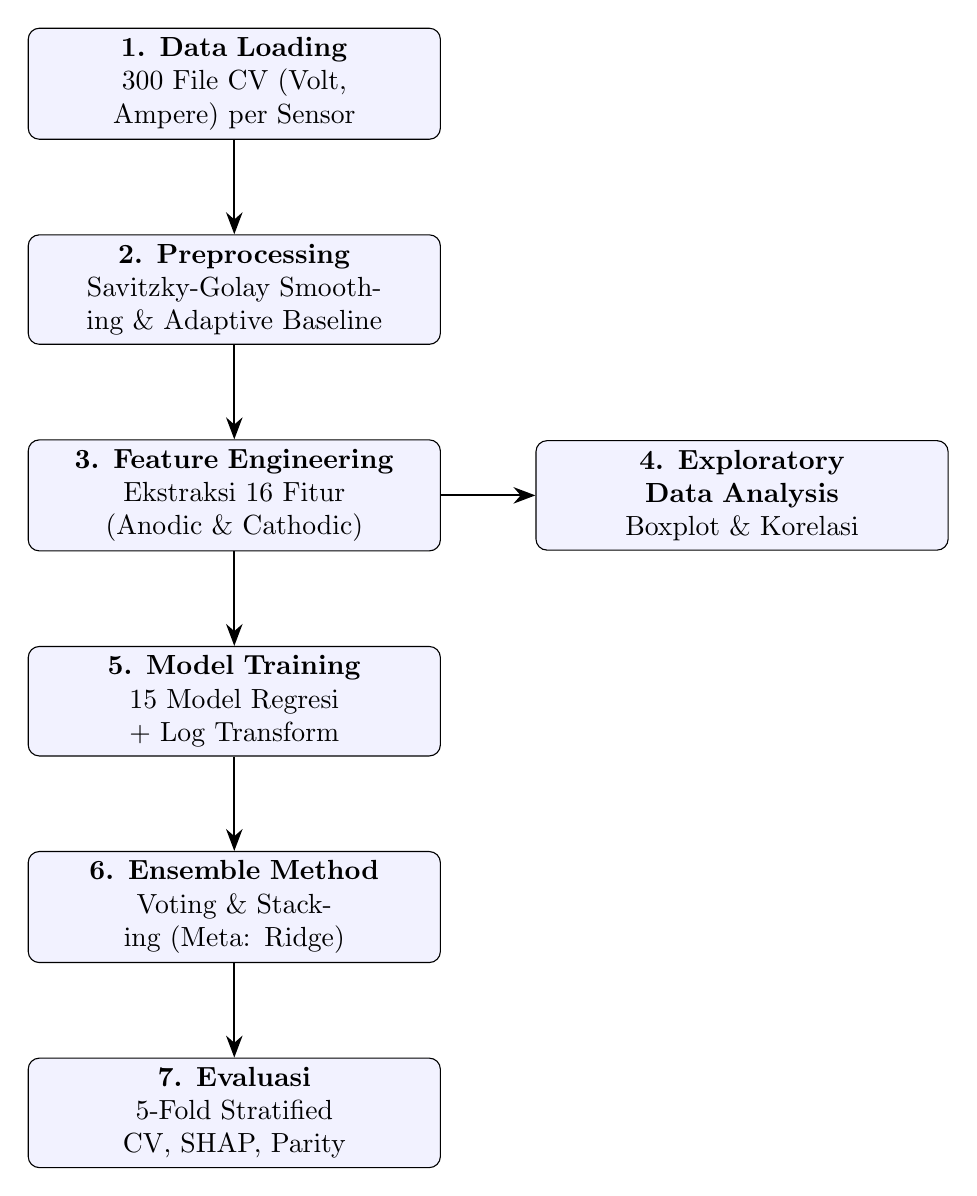
\begin{tikzpicture}[
        node distance=1.2cm and 1.2cm,
        box/.style={rectangle, draw, rounded corners, text width=5cm, align=center, minimum height=1cm, fill=blue!5},
        arrow/.style={-{Stealth[scale=1.2]}, thick}
        ]
        
        \node (data) [box] {\textbf{1. Data Loading} \\ 300 File CV (Volt, Ampere) per Sensor};
        \node (prep) [box, below=of data] {\textbf{2. Preprocessing} \\ Savitzky-Golay Smoothing \& Adaptive Baseline};
        \node (feat) [box, below=of prep] {\textbf{3. Feature Engineering} \\ Ekstraksi 16 Fitur (Anodic \& Cathodic)};
        \node (eda) [box, right=of feat] {\textbf{4. Exploratory Data Analysis} \\ Boxplot \& Korelasi};
        \node (model) [box, below=of feat] {\textbf{5. Model Training} \\ 15 Model Regresi + Log Transform};
        \node (ensemble) [box, below=of model] {\textbf{6. Ensemble Method} \\ Voting \& Stacking (Meta: Ridge)};
        \node (eval) [box, below=of ensemble] {\textbf{7. Evaluasi} \\ 5-Fold Stratified CV, SHAP, Parity};
        
        \draw [arrow] (data) -- (prep);
        \draw [arrow] (prep) -- (feat);
        \draw [arrow] (feat) -- (model);
        \draw [arrow] (feat) -- (eda);
        \draw [arrow] (model) -- (ensemble);
        \draw [arrow] (ensemble) -- (eval);
    \end{tikzpicture}
    \caption{Diagram Alir Pipeline Pemrosesan Sinyal dan Machine Learning}
\end{figure}

\section{HASIL VISUALISASI DAN EVALUASI}

\subsection{Eksplorasi Data dan Deskripsi Fitur (EDA)}
Tabel berikut merangkum deskripsi persebaran nilai ekstraksi dari 16 fitur Dual-Peak pada kedua instrumen:
\begin{table}[H]\n\centering\n\caption{Deskripsi Fitur Sensor LC (Setelah Imputasi)}\n\label{tab:lc_stats}\n\resizebox{\textwidth}{!}{\n\begin{tabular}{@{}lr@{}}\n\toprule\n\textbf{Fitur/Model} & \textbf{mean	std	min	50%	max
ppm	208.125000	309.341801	0.000000	50.000000	1000.000000
upper_Ip_mean	8.430539	19.538610	0.709749	2.834180	88.769639
upper_Ip_std	0.750218	0.904011	0.086310	0.450511	7.184330
upper_Ep_mean	-0.541523	0.041233	-0.620000	-0.518750	-0.500000
upper_Ep_std	0.014049	0.016032	0.000000	0.006960	0.058830
upper_Area_mean	0.500604	1.220068	0.042642	0.155283	5.612287
upper_FWHM_mean	0.057539	0.008969	0.040000	0.055000	0.100000
upper_skewness	0.043566	0.525391	-1.426912	0.058839	1.751070
upper_kurtosis	-0.678789	0.906082	-1.505126	-1.166908	2.615111
lower_Ip_mean	43.997366	43.688143	17.973174	28.516098	217.792284
lower_Ip_std	1.361553	1.908715	0.137375	0.739836	18.201608
lower_Ep_mean	-0.795706	0.014585	-0.800000	-0.800000	-0.642500
lower_Ep_std	0.002067	0.004893	0.000000	0.000000	0.062837
lower_Area_mean	6.567825	6.075467	3.051835	4.362758	31.629153
lower_FWHM_mean	0.000000	0.000000	0.000000	0.000000	0.000000
lower_skewness	0.390287	0.470942	-1.494845	0.555018	1.357457
lower_kurtosis	-0.195462	0.854349	-1.211072	-0.490465	4.085955} \\\n\midrule\n\bottomrule\n\end{tabular}\n}\n\end{table}\n
\begin{table}[H]\n\centering\n\caption{Deskripsi Fitur Sensor PS (Setelah Imputasi)}\n\label{tab:ps_stats}\n\resizebox{\textwidth}{!}{\n\begin{tabular}{@{}lr@{}}\n\toprule\n\textbf{Fitur/Model} & \textbf{mean	std	min	50%	max
ppm	208.632371	309.812736	0.000000	40.000000	1000.000000
upper_Ip_mean	13.557990	9.752524	4.150540	11.993419	94.960037
upper_Ip_std	0.676910	1.775550	0.016749	0.261878	27.381340
upper_Ep_mean	-0.612767	0.080238	-0.770198	-0.640097	-0.508745
upper_Ep_std	0.008037	0.016908	0.000000	0.003310	0.105171
upper_Area_mean	2.334686	1.302799	0.579185	2.035140	10.233456
upper_FWHM_mean	0.162820	0.019558	0.080062	0.158873	0.230179
upper_skewness	-1.385005	0.685230	-2.978713	-1.512334	0.879842
upper_kurtosis	2.080580	1.988813	-1.457411	1.778225	8.892112
lower_Ip_mean	45.918064	19.450620	27.092913	40.202563	192.723356
lower_Ip_std	1.446210	3.141528	0.012246	0.393147	47.318024
lower_Ep_mean	-0.876745	0.018522	-0.890292	-0.880284	-0.772700
lower_Ep_std	0.001319	0.004569	0.000000	0.000000	0.045035
lower_Area_mean	8.103872	3.609664	5.014272	7.403152	38.853195
lower_FWHM_mean	0.000000	0.000000	0.000000	0.000000	0.000000
lower_skewness	-0.117577	0.512964	-1.631632	-0.056581	0.649130
lower_kurtosis	-0.394841	0.643521	-1.328502	-0.560666	2.120147} \\\n\midrule\n\bottomrule\n\end{tabular}\n}\n\end{table}\n

Heatmap korelasi memperlihatkan interdependensi kuat antara variabel \textit{current} (I) dengan besaran konsentrasi.
\begin{figure}[H]
    \centering
    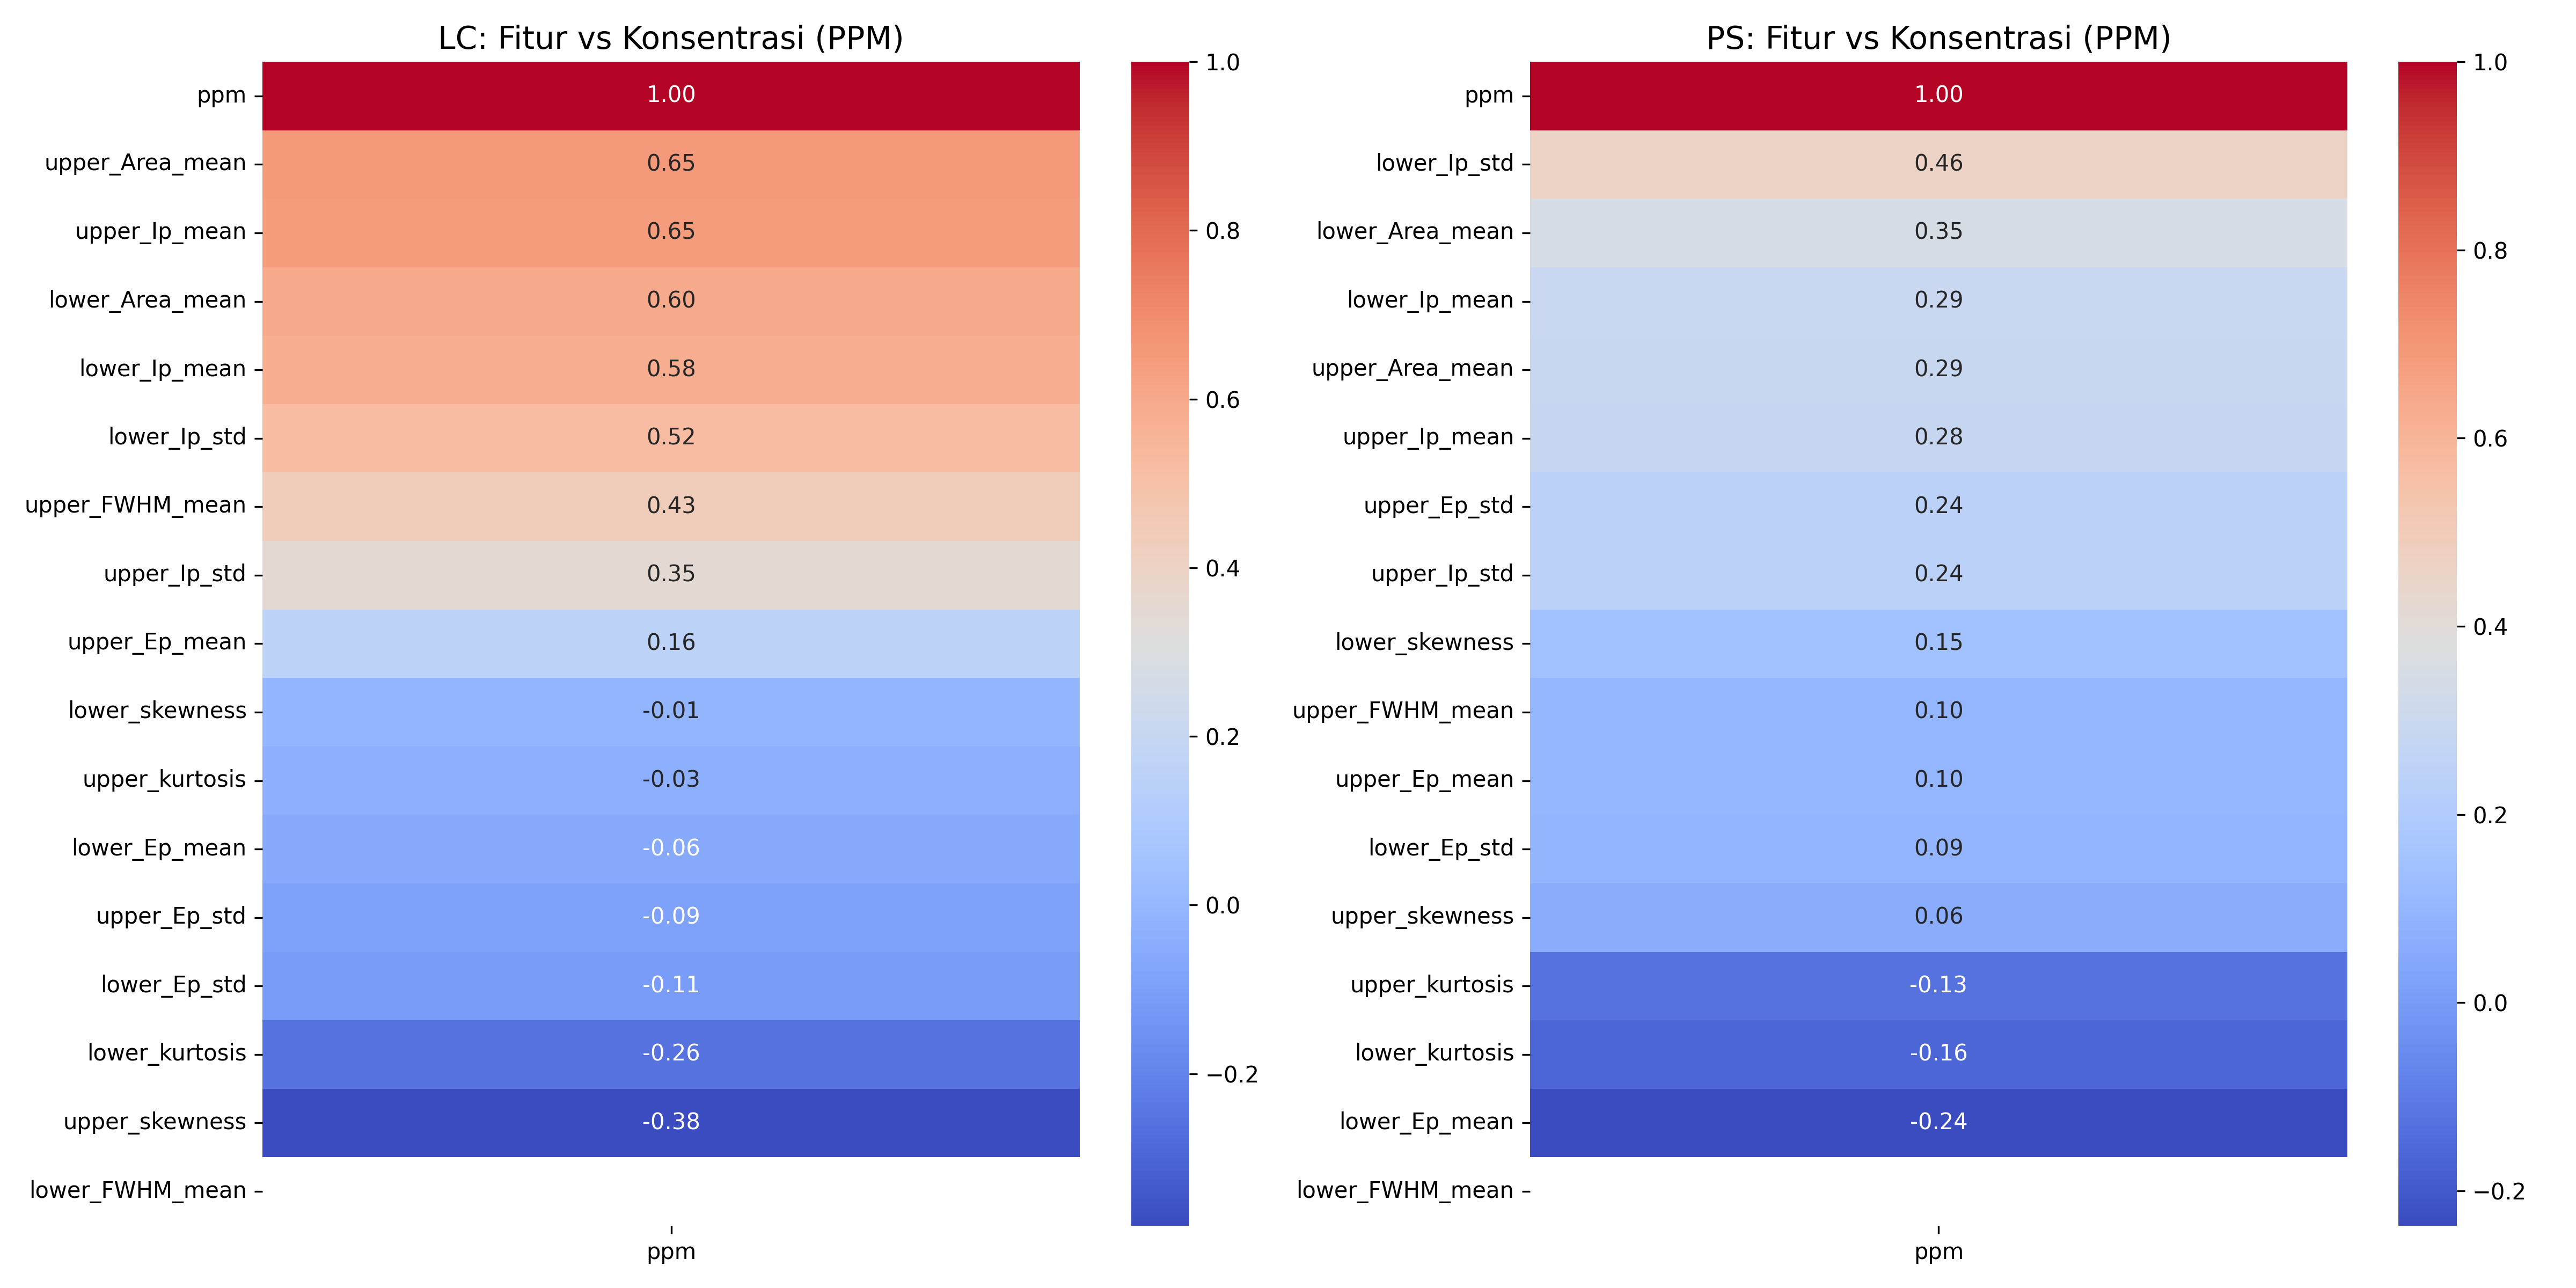
\includegraphics[width=0.9\textwidth]{output/phase3_korelasi.png}
    \caption{Heatmap Korelasi Pearson: 16 Fitur terhadap Konsentrasi (PPM)}
\end{figure}

\begin{figure}[H]
    \centering
    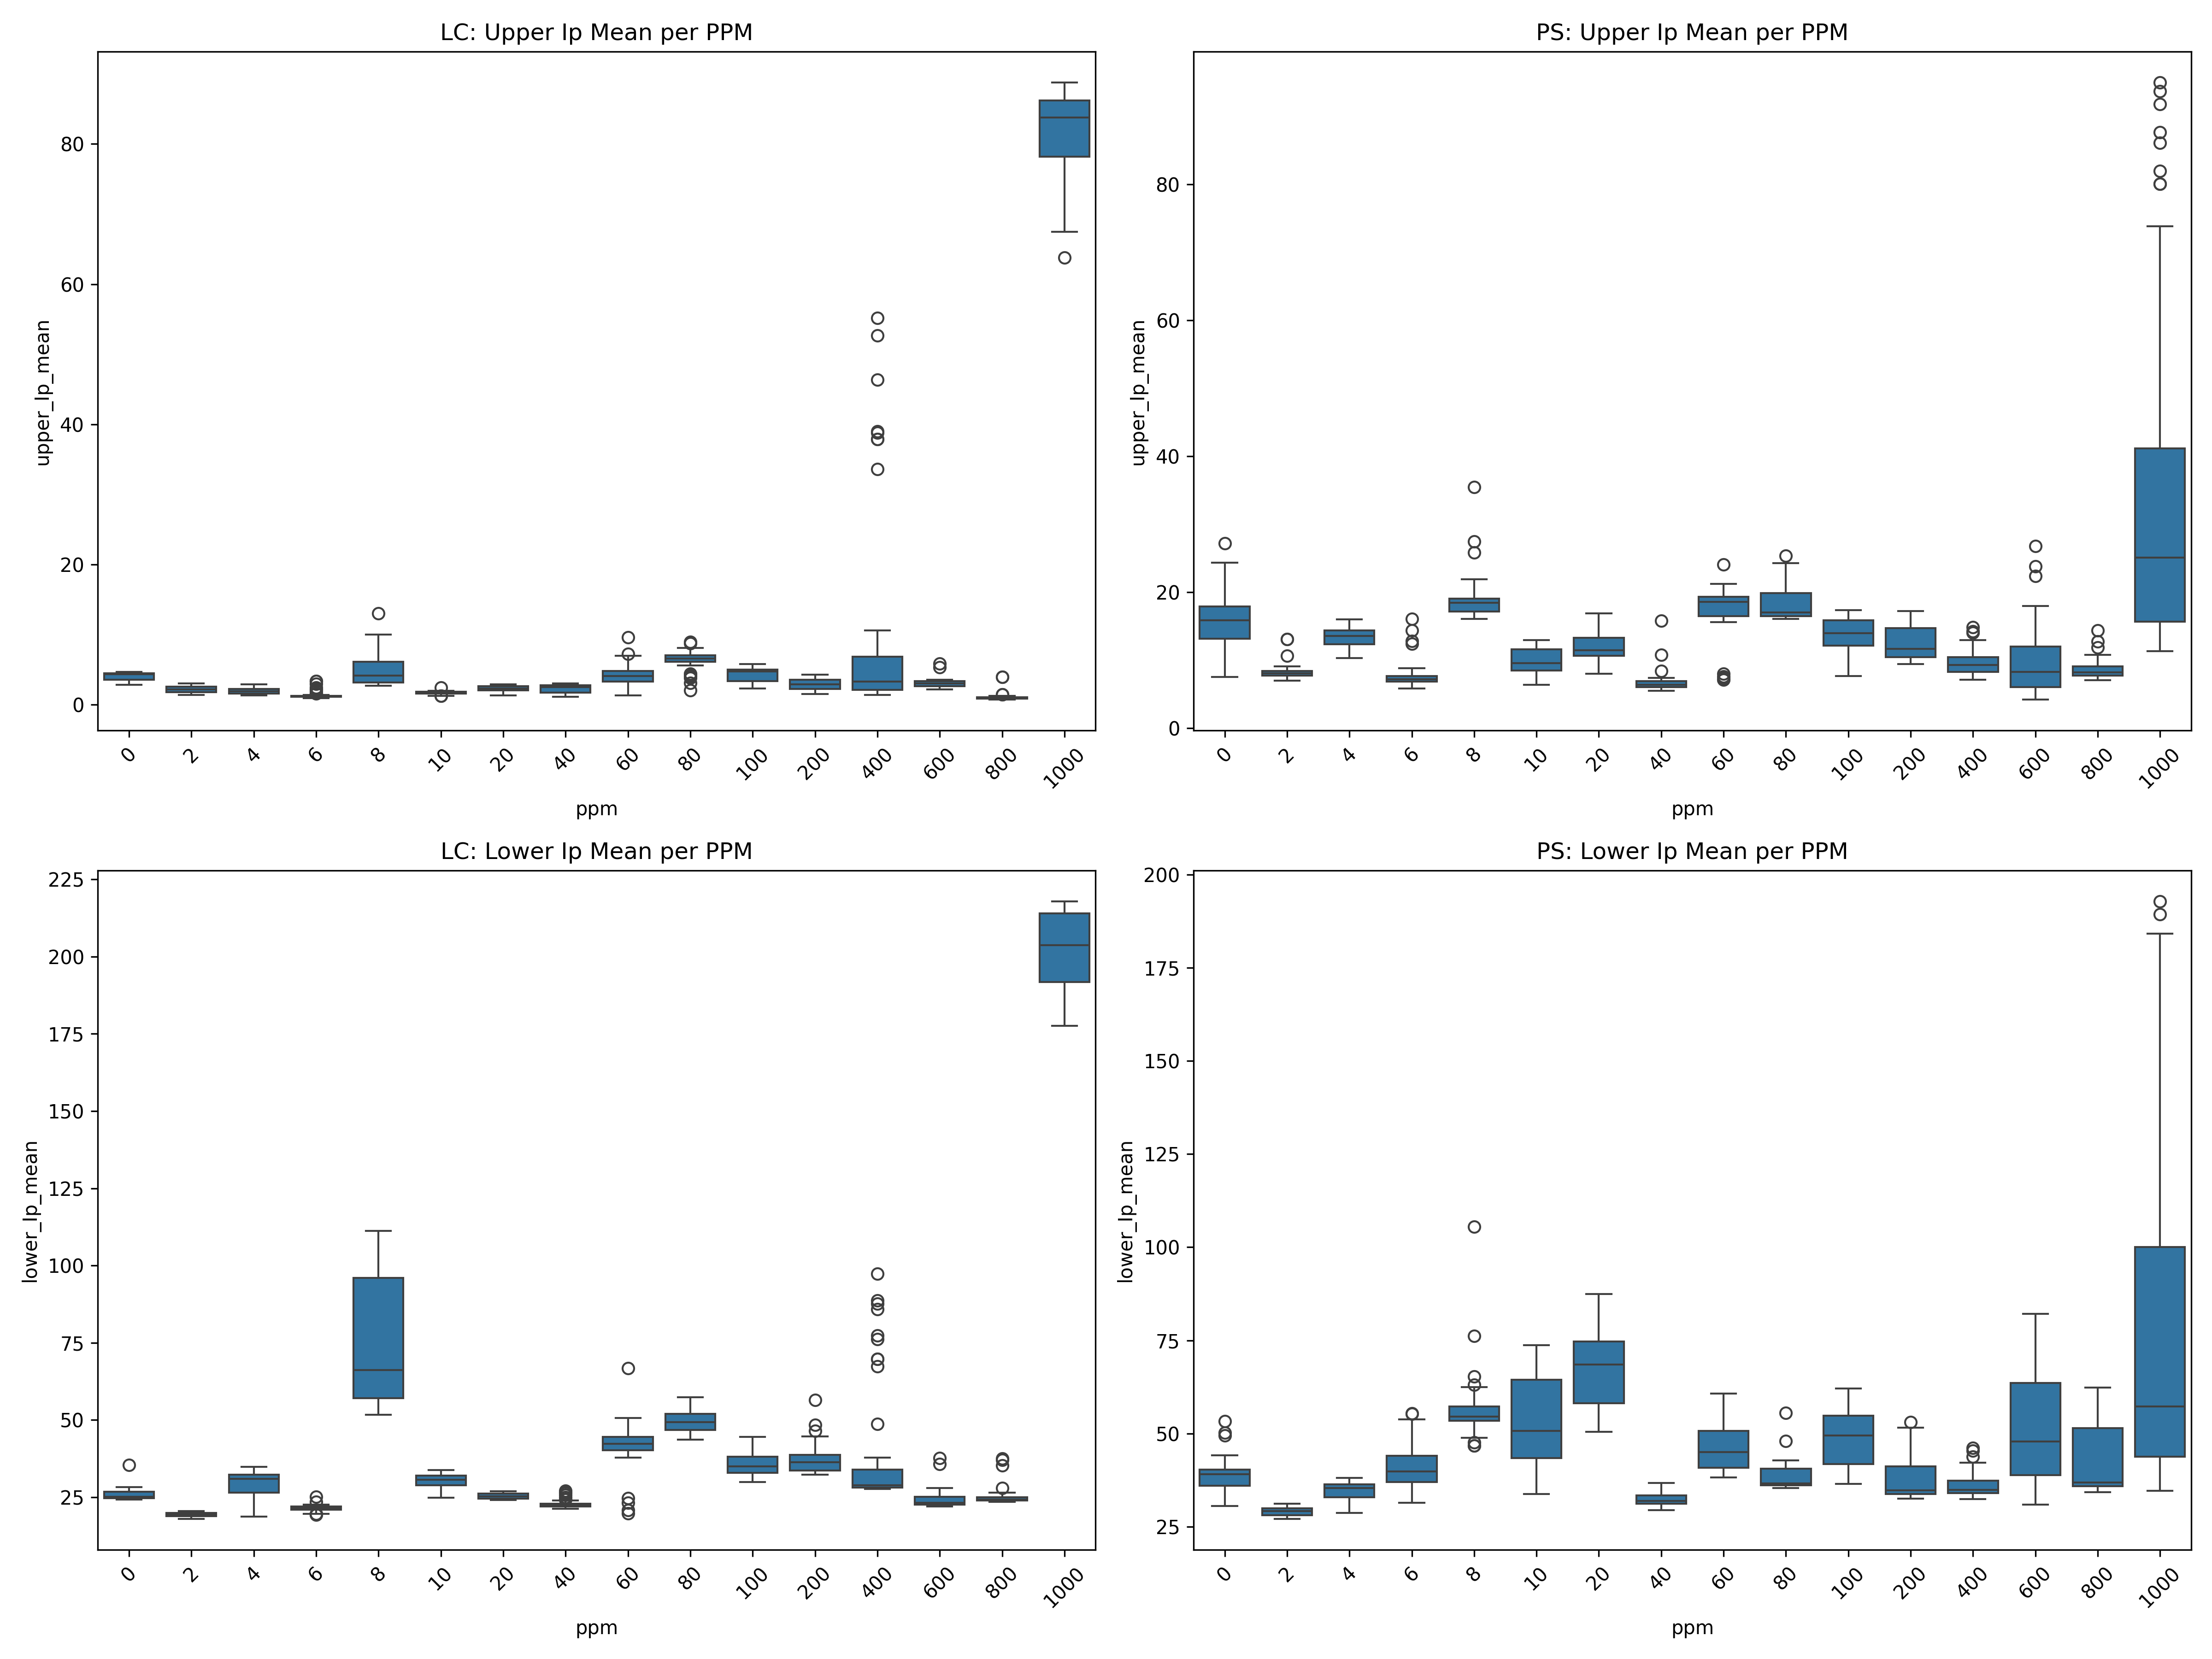
\includegraphics[width=0.9\textwidth]{output/phase3_boxplot_ppm.png}
    \caption{Boxplot Sebaran Arus Puncak (Ip Mean) Berdasarkan Level Konsentrasi}
\end{figure}

\begin{figure}[H]
    \centering
    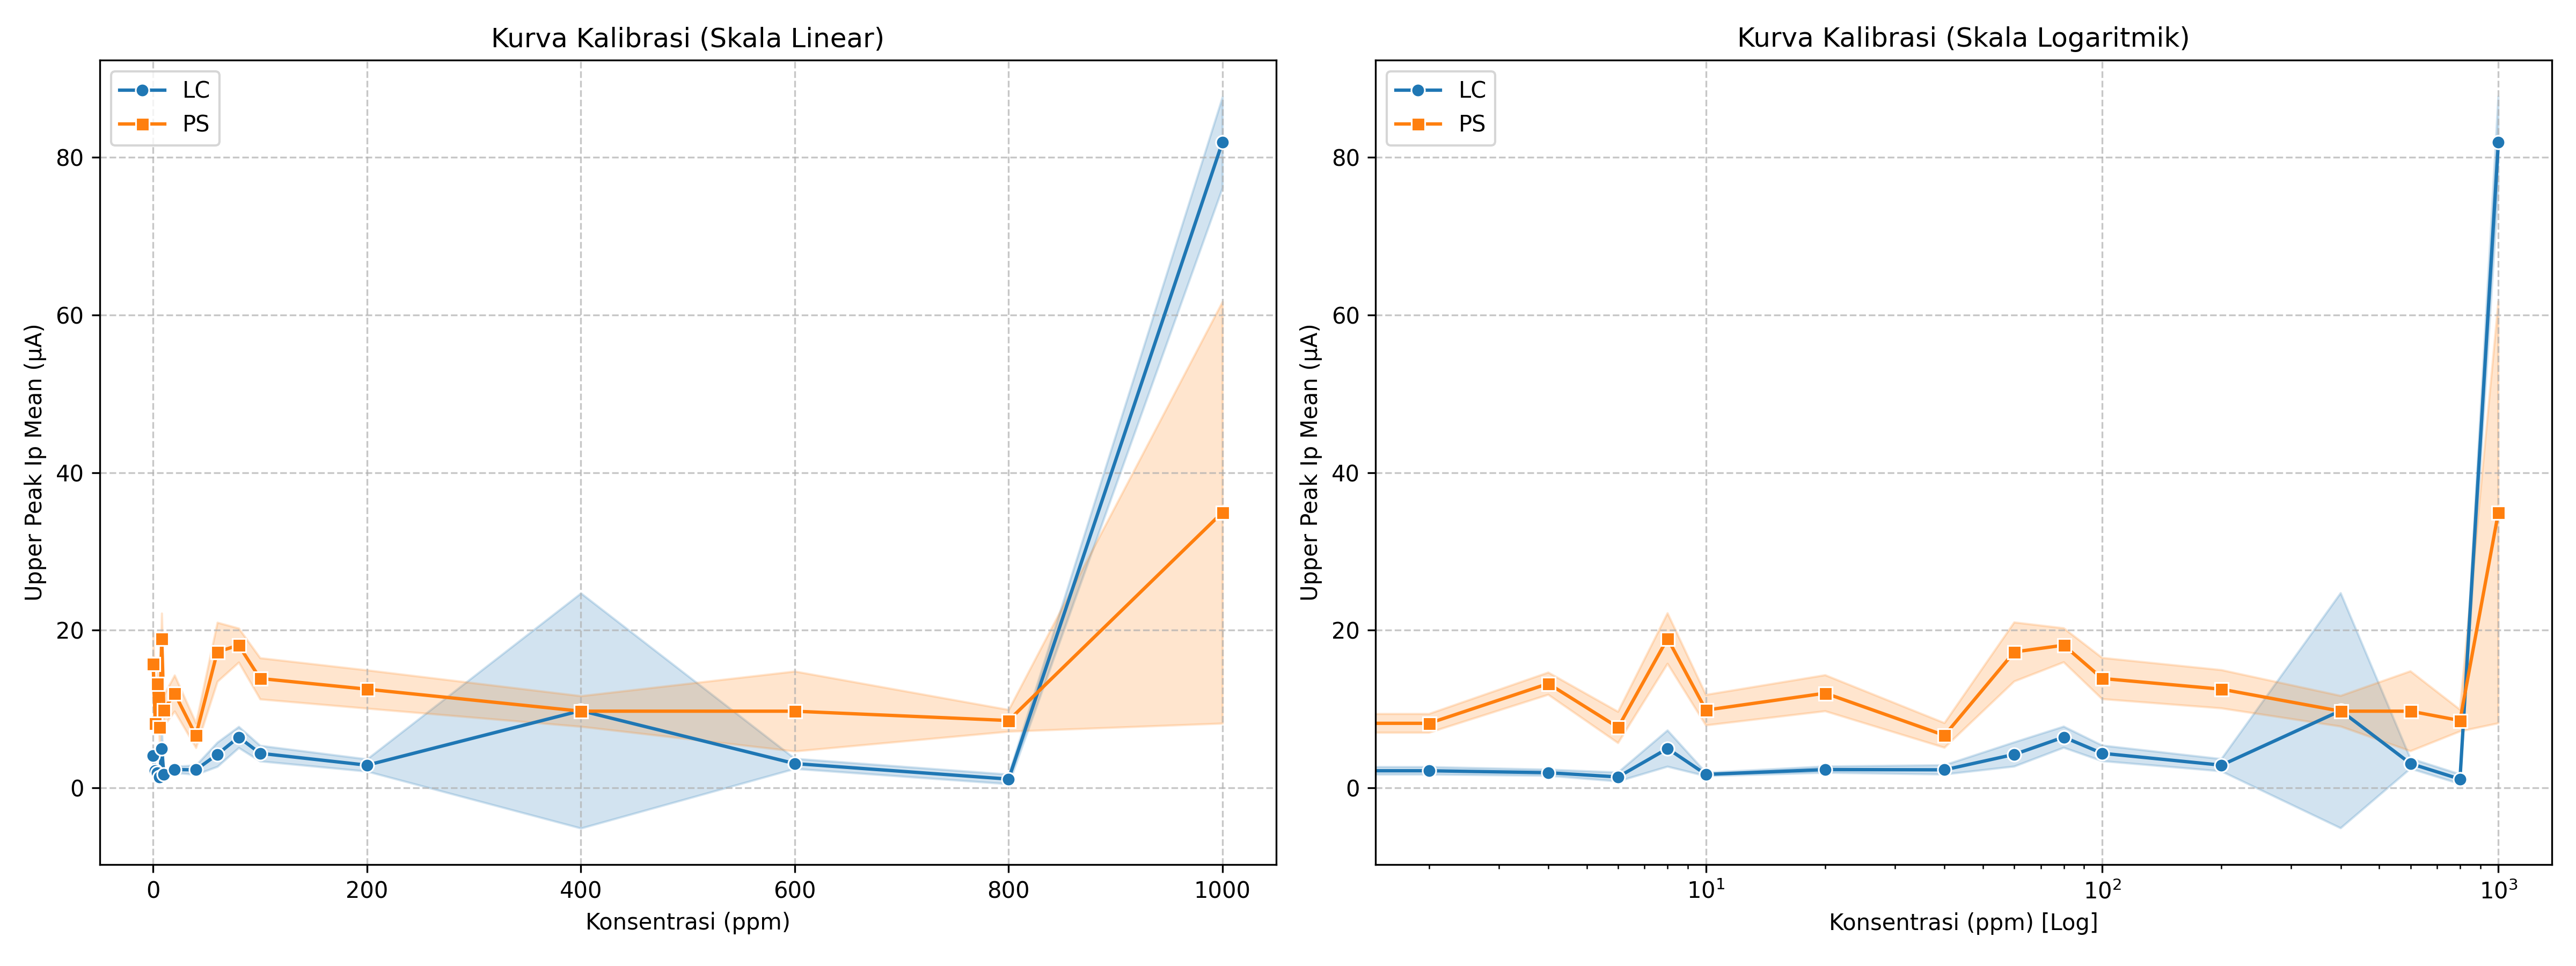
\includegraphics[width=0.9\textwidth]{output/phase3_calibration_curve.png}
    \caption{Kurva Kalibrasi Sensor LC vs PS (Skala Linear dan Logaritmik)}
\end{figure}

\subsection{Evaluasi Metrik Performa Model}
Pengujian menggunakan metode \textit{Stratified 5-Fold CV} memastikan distribusi rentang konsentrasi merata di setiap *fold* evaluasi. Berikut adalah tabel komparasi peringkat seluruh model yang dilatih:

\begin{table}[H]\n\centering\n\caption{Peringkat Evaluasi Model Regresi (Sensor LC)}\n\label{tab:lc_models}\n\resizebox{\textwidth}{!}{\n\begin{tabular}{@{}lr@{}}\n\toprule\n\textbf{Fitur/Model} & \textbf{R2	RMSE	MAE	MAPE
11. TabICLv2	9.970486e-01	1.668396e+01	2.699991e+00	0.017123
10. CatBoost_Tuned	9.482524e-01	6.957326e+01	2.624783e+01	0.169911
7. ExtraTrees	9.437108e-01	7.223605e+01	2.440696e+01	0.169095
8. XGBoost_Tuned	9.429786e-01	7.234562e+01	2.522889e+01	0.191863
6. RandomForest	9.381329e-01	7.361420e+01	2.458002e+01	0.209213
9. LightGBM_Tuned	9.310752e-01	7.957052e+01	3.340116e+01	0.230981
13. CAFF_Tuned	8.913909e-01	1.009321e+02	4.737880e+01	0.288011
12. CAFF	7.952697e-01	1.354709e+02	6.870707e+01	0.422156
5. SVR	6.738770e-01	1.749995e+02	7.972337e+01	0.794115
3. ElasticNet	2.953186e-01	2.592770e+02	1.463610e+02	2.493792
2. Ridge	-1.111416e+00	3.845932e+02	1.534755e+02	2.437840
1. LinearRegression	-9.532611e+00	7.618929e+02	2.267585e+02	2.984260
4. PolyRidge	-8.668431e+11	1.287309e+08	1.439236e+07	38380.665810} \\\n\midrule\n\bottomrule\n\end{tabular}\n}\n\end{table}\n
\begin{table}[H]\n\centering\n\caption{Peringkat Evaluasi Model Regresi (Sensor PS)}\n\label{tab:ps_models}\n\resizebox{\textwidth}{!}{\n\begin{tabular}{@{}lr@{}}\n\toprule\n\textbf{Fitur/Model} & \textbf{R2	RMSE	MAE	MAPE
11. TabICLv2	9.918507e-01	2.620922e+01	4.885186e+00	3.541805e-02
10. CatBoost_Tuned	8.625573e-01	1.133155e+02	4.292904e+01	2.876881e-01
9. LightGBM_Tuned	8.078226e-01	1.353222e+02	5.543142e+01	4.415865e-01
7. ExtraTrees	8.071439e-01	1.346568e+02	4.501273e+01	2.706228e-01
8. XGBoost_Tuned	7.945163e-01	1.387889e+02	5.297698e+01	3.223620e-01
6. RandomForest	7.710746e-01	1.477430e+02	5.340337e+01	4.327345e-01
12. CAFF	6.566113e-01	1.812861e+02	8.329385e+01	4.504011e-01
13. CAFF_Tuned	4.943275e-01	2.198866e+02	1.079127e+02	4.533558e-01
5. SVR	-3.686583e+00	5.479590e+02	1.281031e+02	5.954777e-01
3. ElasticNet	-7.057141e+03	1.188534e+04	1.089717e+03	3.660321e+00
1. LinearRegression	-2.483284e+08	2.184290e+06	1.733671e+05	3.102263e+02
2. Ridge	-2.540692e+08	2.209366e+06	1.753499e+05	3.137796e+02
4. PolyRidge	-1.928897e+102	1.925144e+53	1.526738e+52	1.629204e+49} \\\n\midrule\n\bottomrule\n\end{tabular}\n}\n\end{table}\n

\begin{figure}[H]
    \centering
    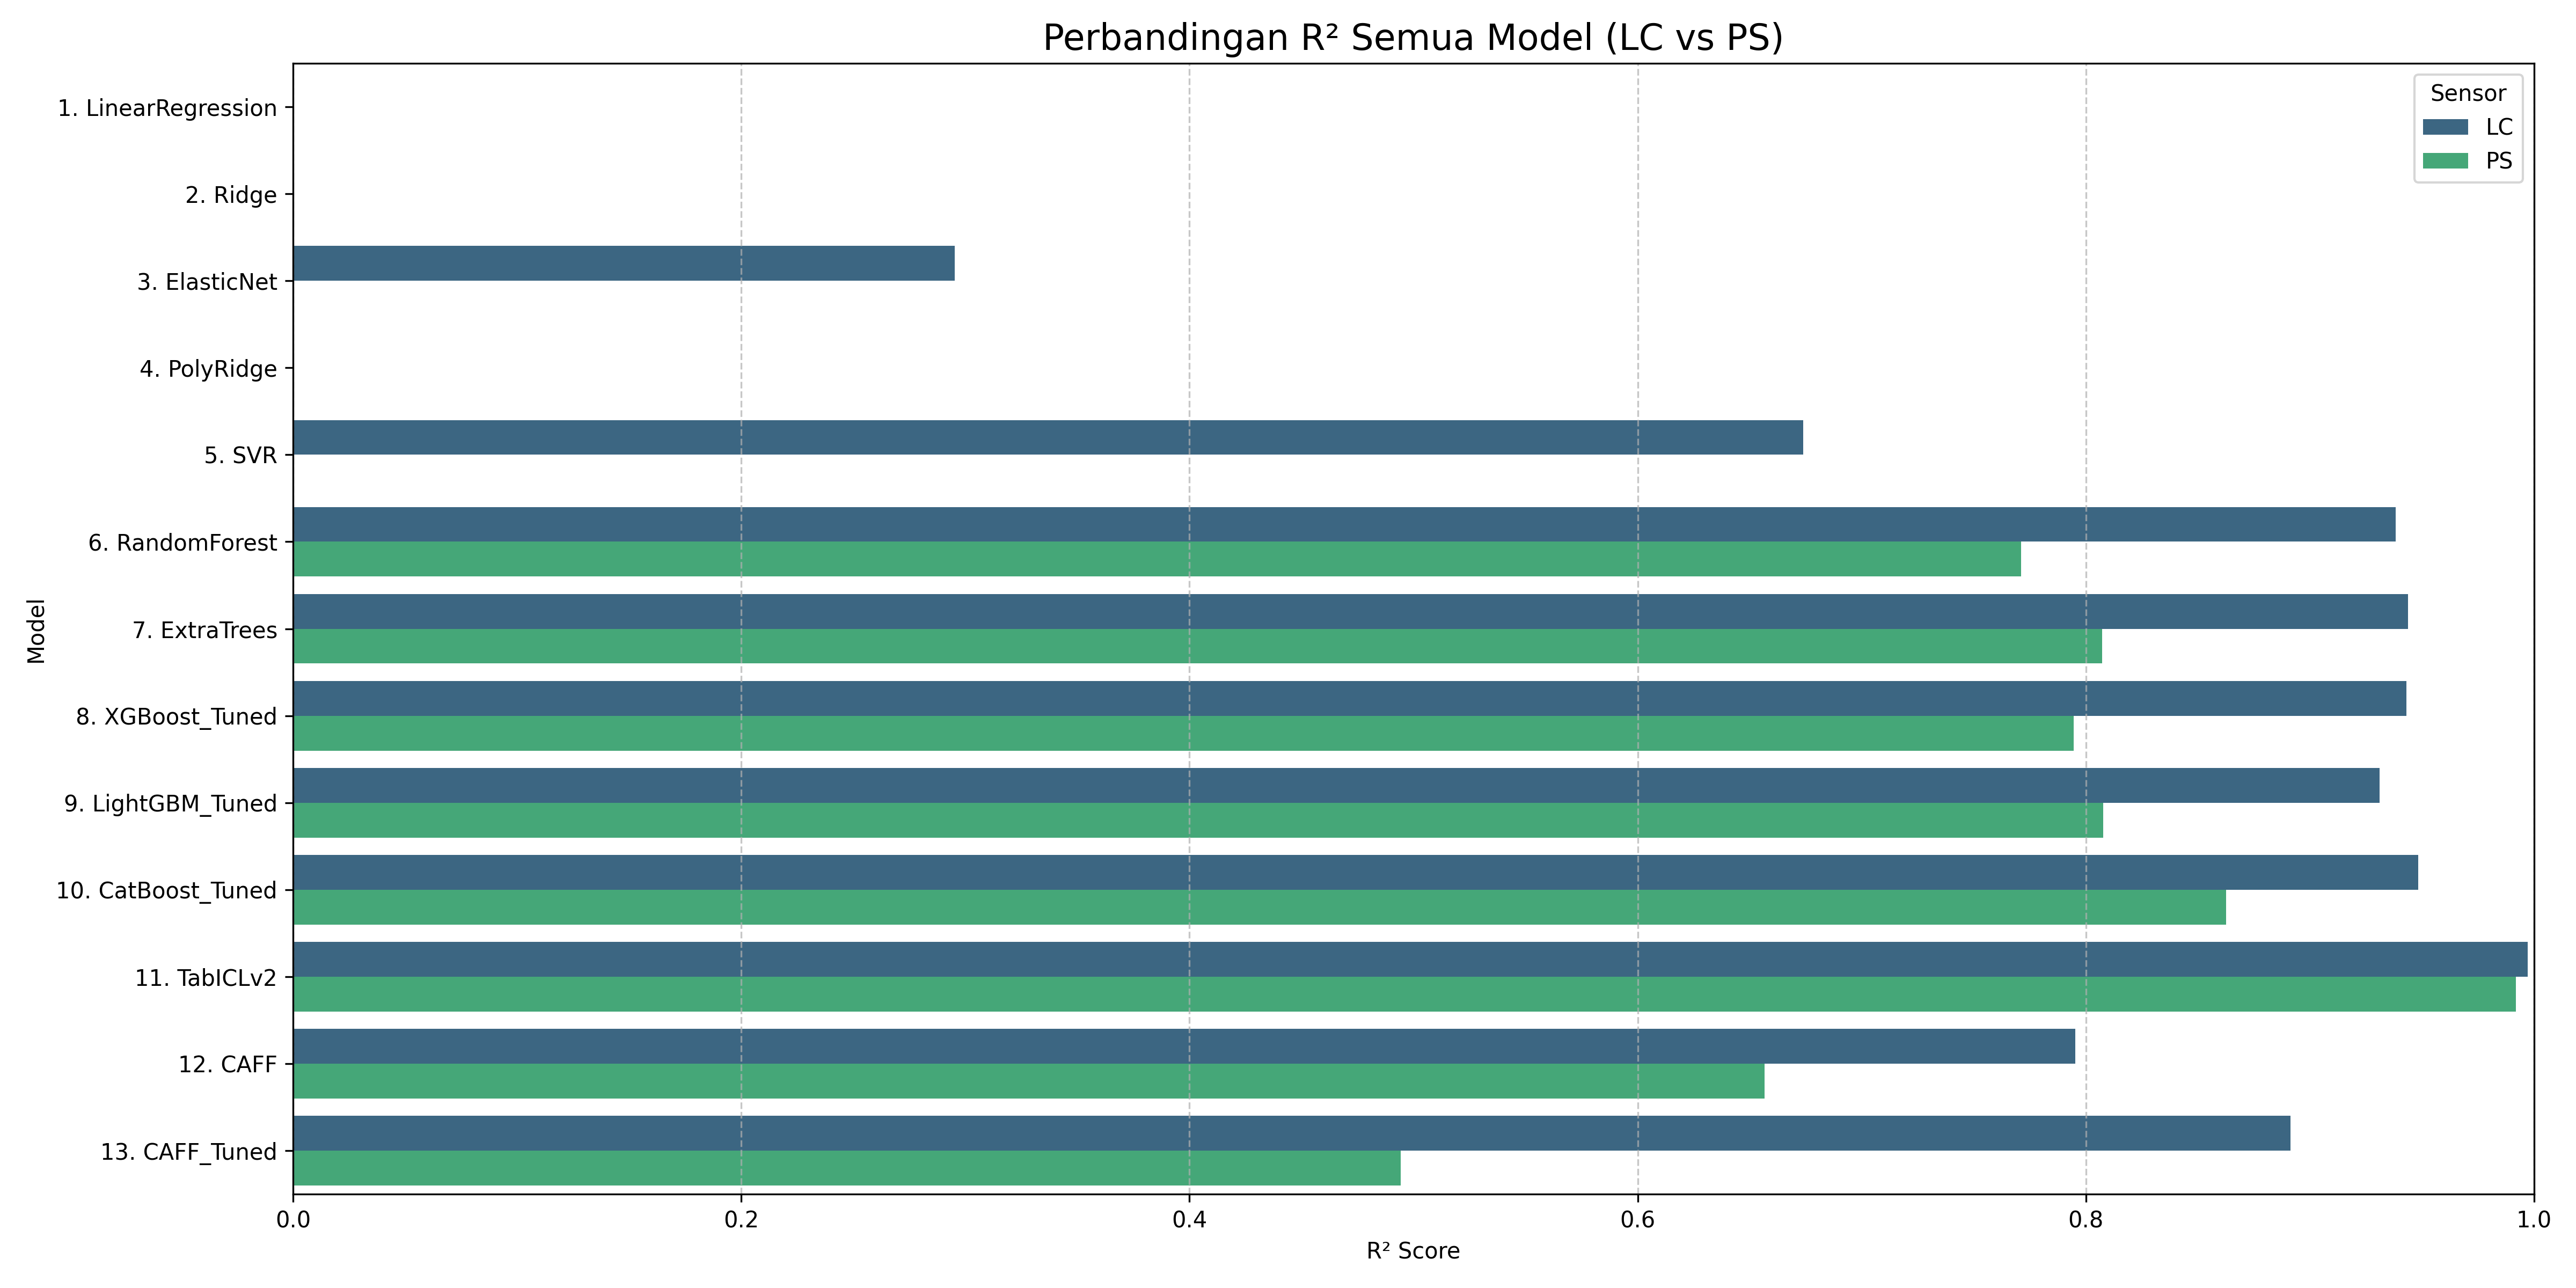
\includegraphics[width=0.9\textwidth]{output/phase6_barchart_r2.png}
    \caption{Perbandingan Metrik $R^2$ Seluruh Model (LC vs PS)}
\end{figure}

\begin{figure}[H]
    \centering
    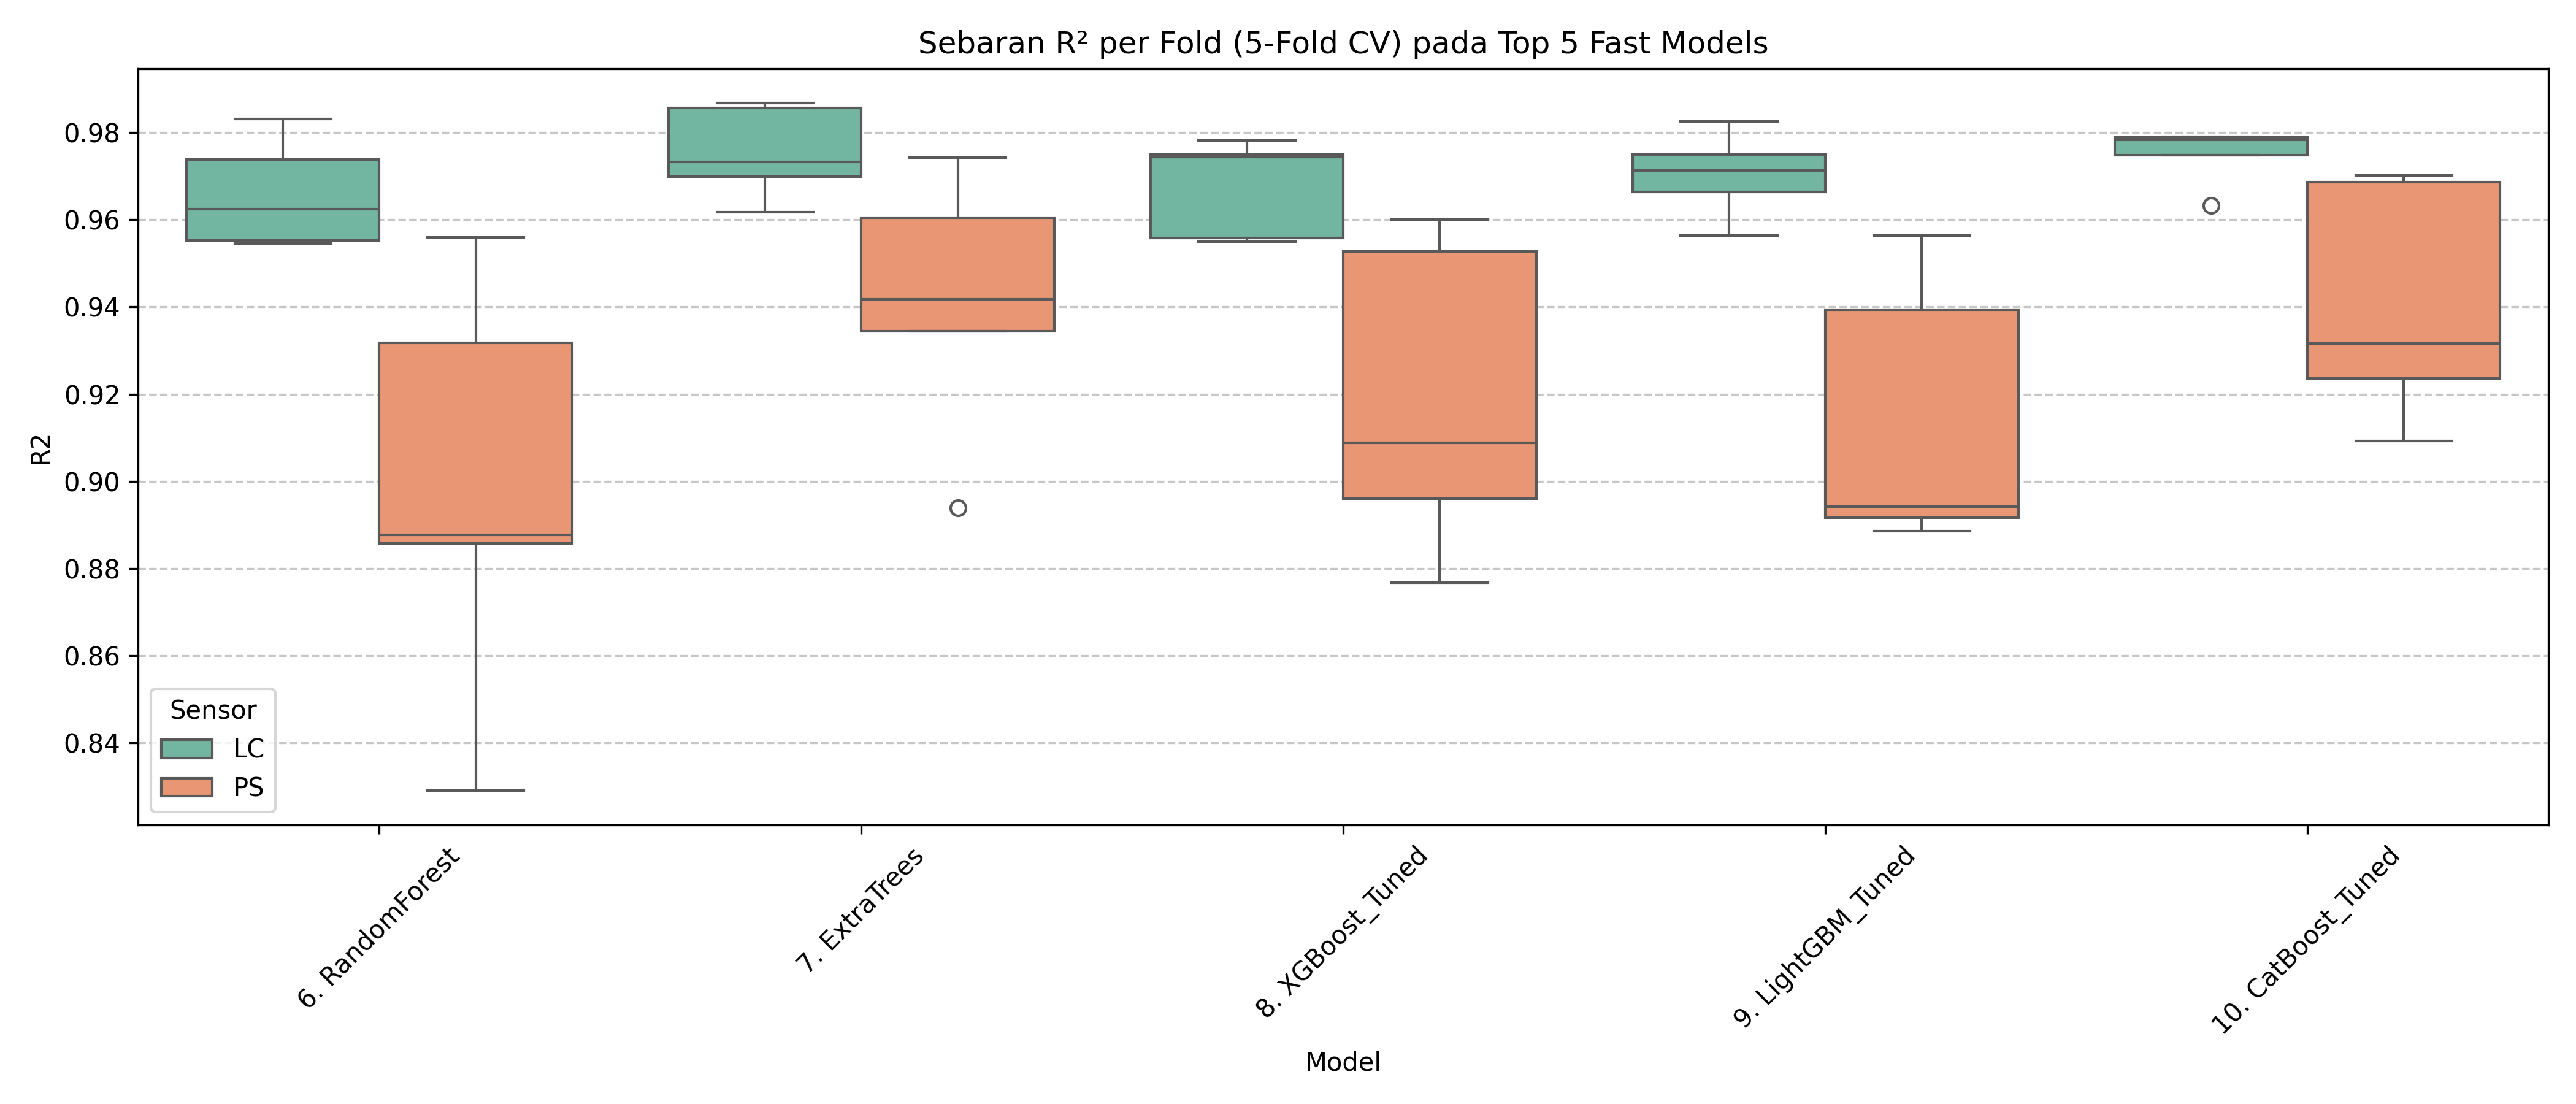
\includegraphics[width=0.9\textwidth]{output/phase6_boxplot_r2_fold.png}
    \caption{Stabilitas $R^2$ per Fold pada Top 5 Model (Stratified 5-Fold CV)}
\end{figure}

\section{PEMBAHASAN DAN ANALISIS HASIL}

\subsection{Ketepatan Prediksi (Parity \& Residual Plot)}
Untuk menginspeksi seberapa besar penyimpangan (*error*) antara nilai aktual dengan prediksi dari model terbaik, kami menggunakan metrik \textit{Parity Plot} dan distribusi rentang \textit{Residual}.

\begin{figure}[H]
    \centering
    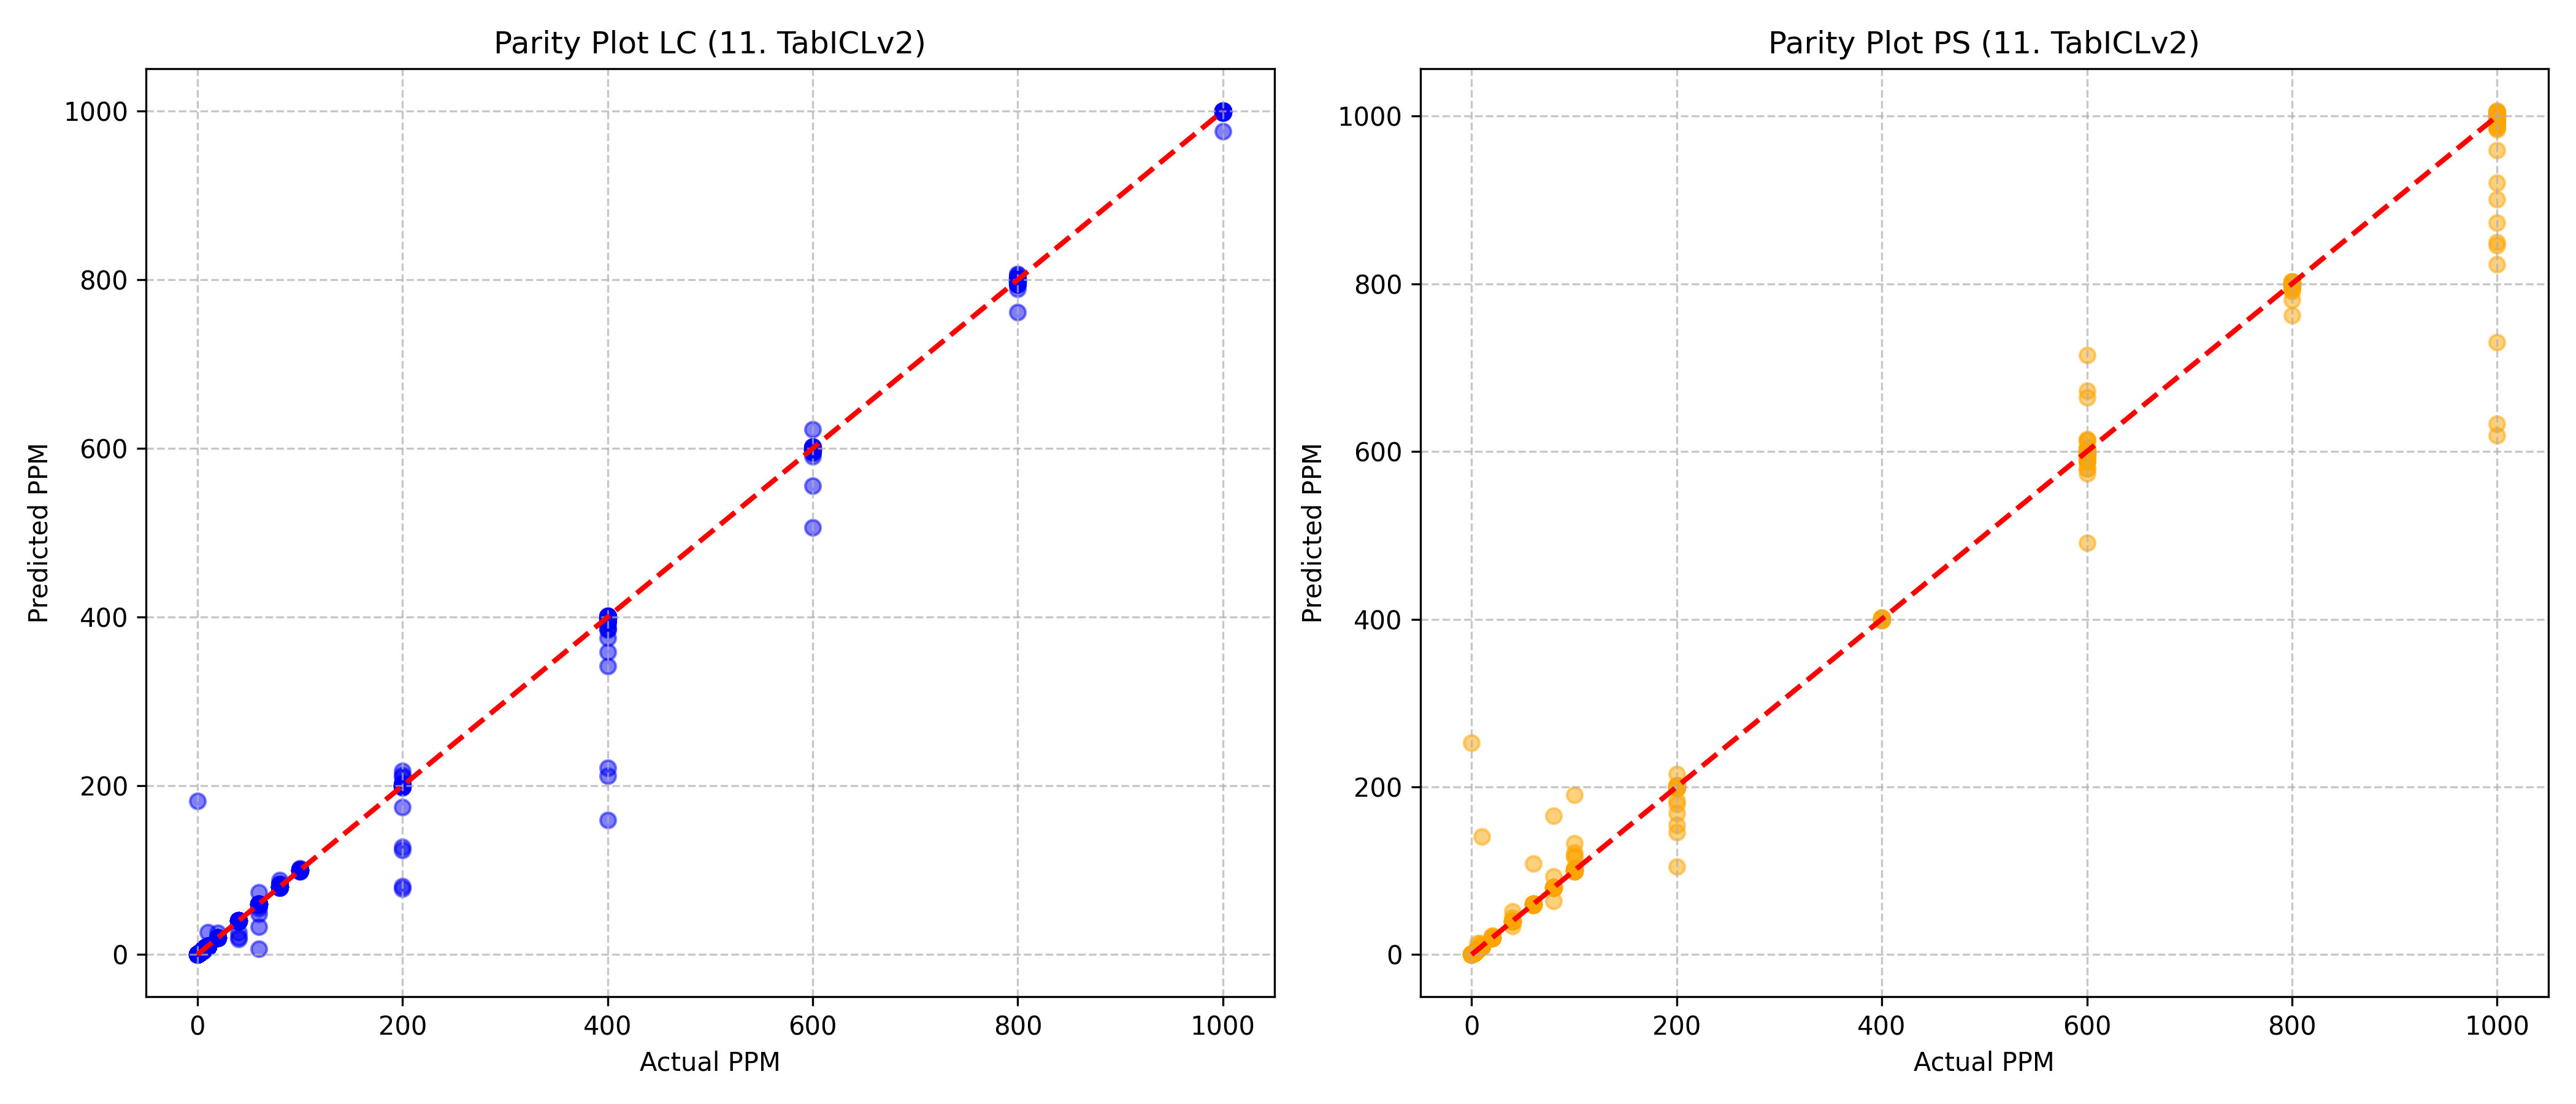
\includegraphics[width=0.9\textwidth]{output/phase6_parity_plot.png}
    \caption{Parity Plot Prediksi Konsentrasi Kadmium dari Model Terbaik}
\end{figure}

\begin{figure}[H]
    \centering
    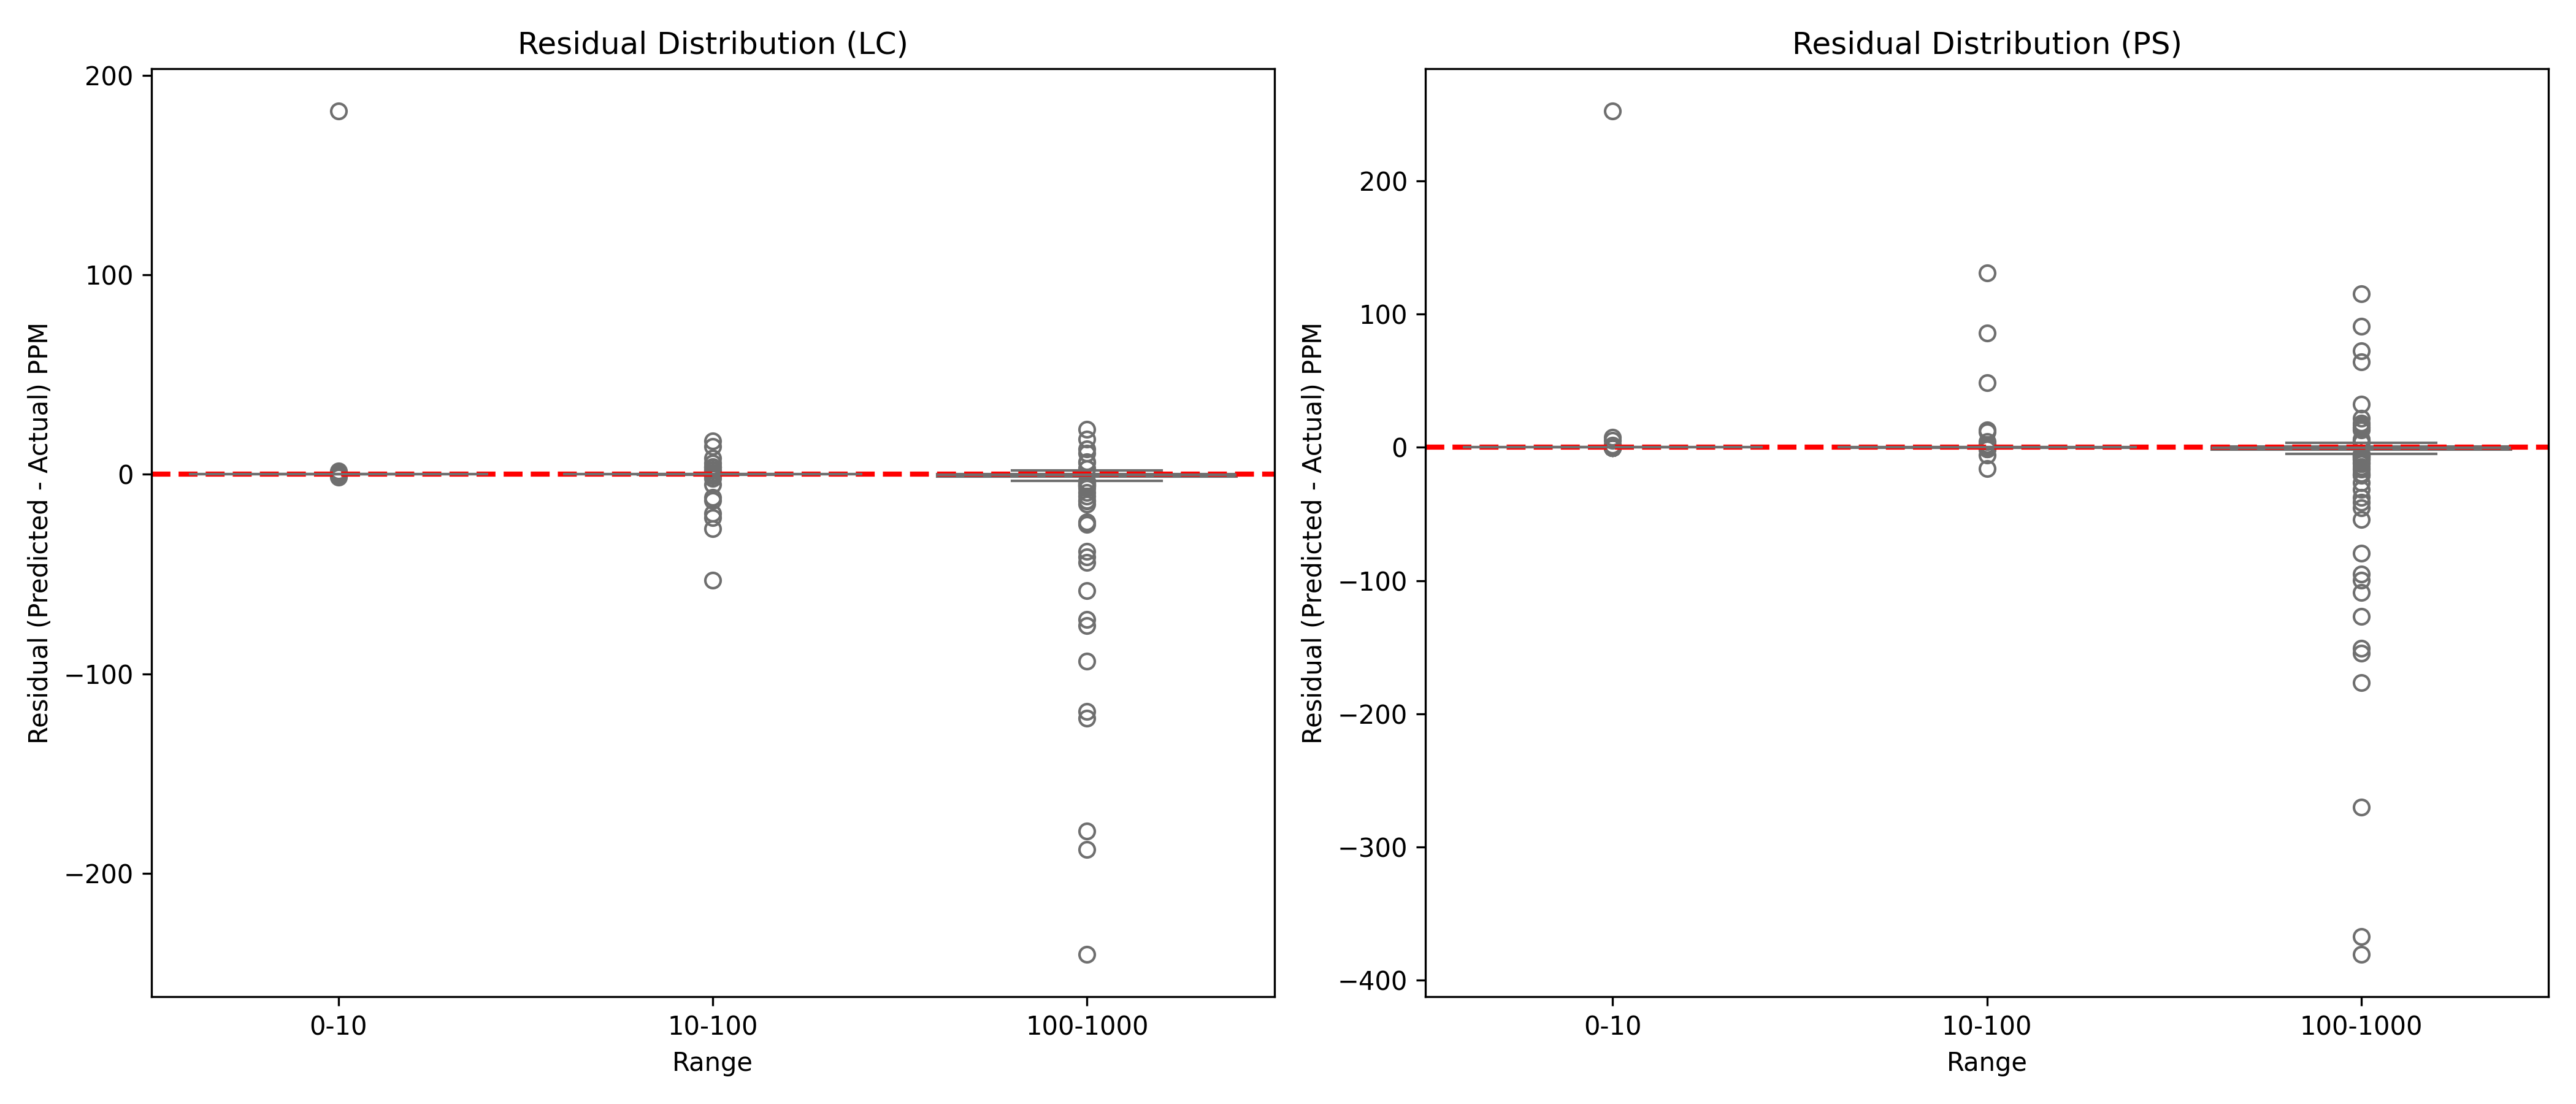
\includegraphics[width=0.9\textwidth]{output/phase6_residual_plot.png}
    \caption{Distribusi Error Residual Berdasarkan Rentang Konsentrasi}
\end{figure}

Residual plot memperlihatkan pelebaran *error* (	extit{heteroscedasticity}) di rentang konsentrasi tinggi (100-1000 ppm) baik di LC maupun PS, dikarenakan sifat elektrokimia yang saturasi (kemacetan transfer massa pada elektrode). Kendati demikian, di rentang kritikal (0-10 ppm) yang krusial untuk deteksi awal tingkat toksisitas air, instrumen LC menunjukan stabilitas prediksi yang sangat presisi dengan garis simpangan yang amat tipis mendekati sumbu nol.

\subsection{Interpretasi Model dengan SHAP}
Pendekatan \textit{SHapley Additive exPlanations} (SHAP)\cite{shap} diterapkan pada model *XGBoost* untuk membedah *Feature Importance* secara transparan.

\begin{figure}[H]
    \centering
    \begin{minipage}{0.48\textwidth}
        \centering
        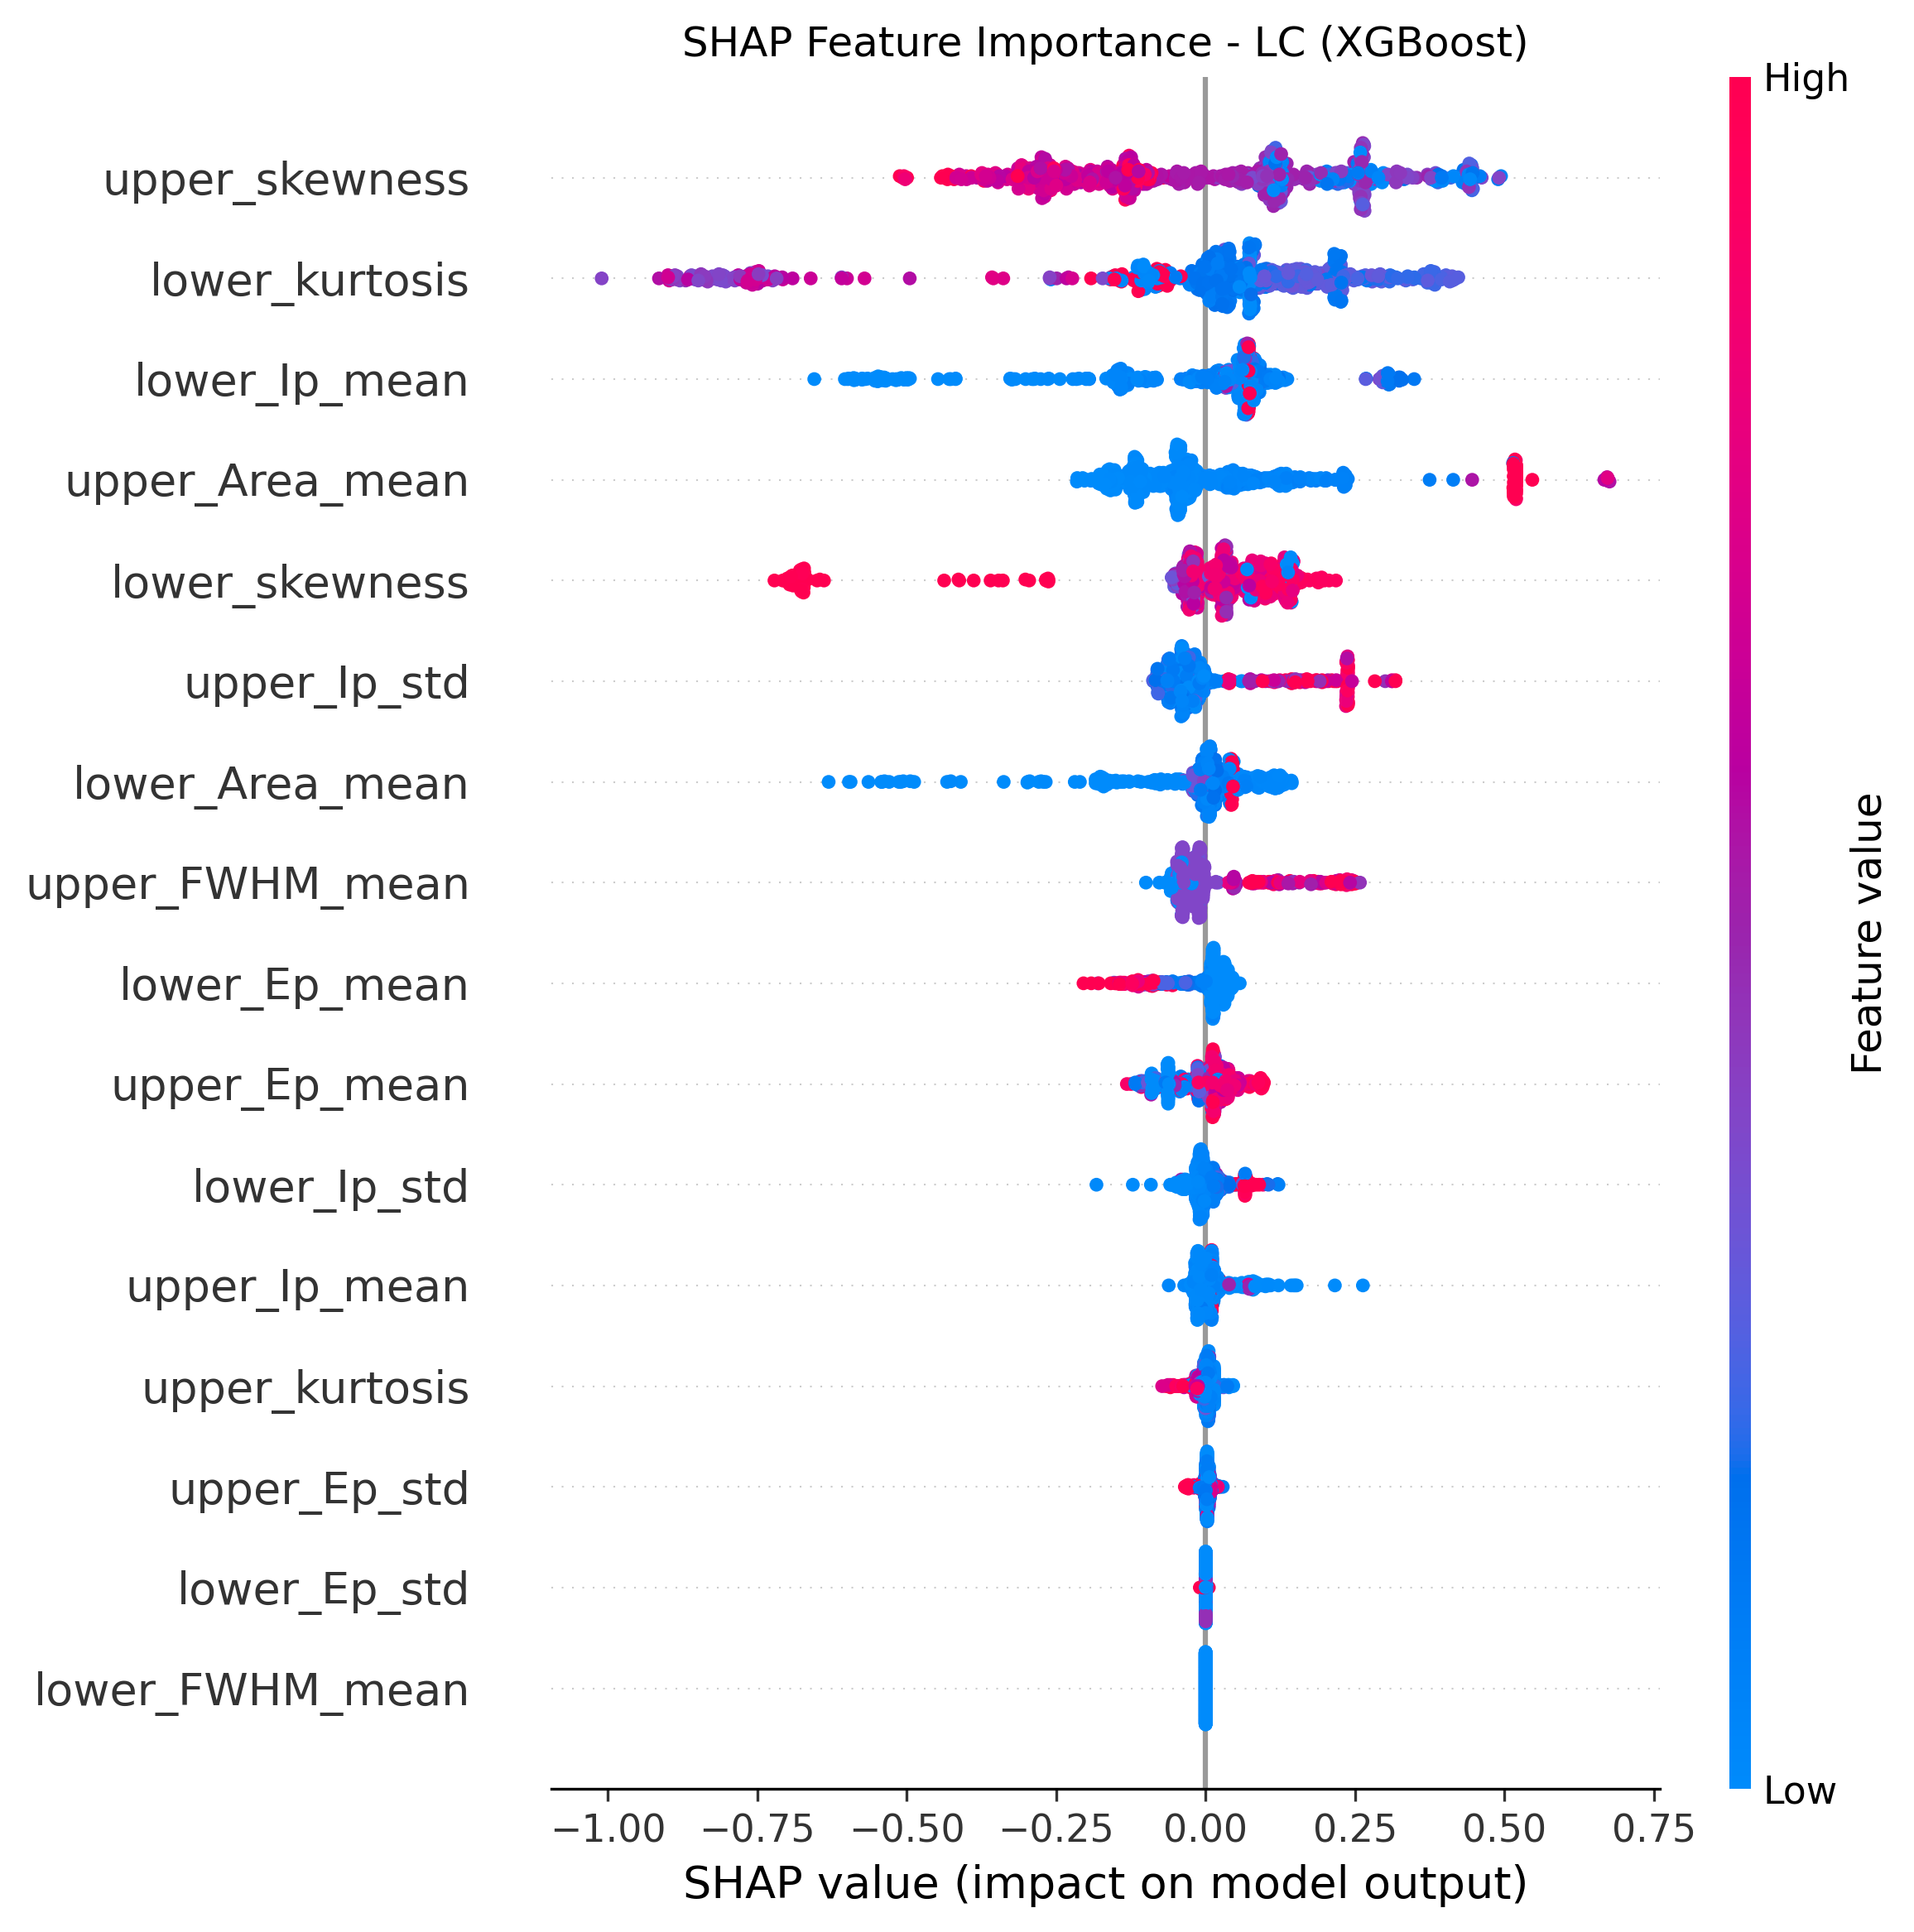
\includegraphics[width=\textwidth]{output/phase6_shap_lc.png}
        \caption{SHAP Summary Plot (LC)}
    \end{minipage}\hfill
    \begin{minipage}{0.48\textwidth}
        \centering
        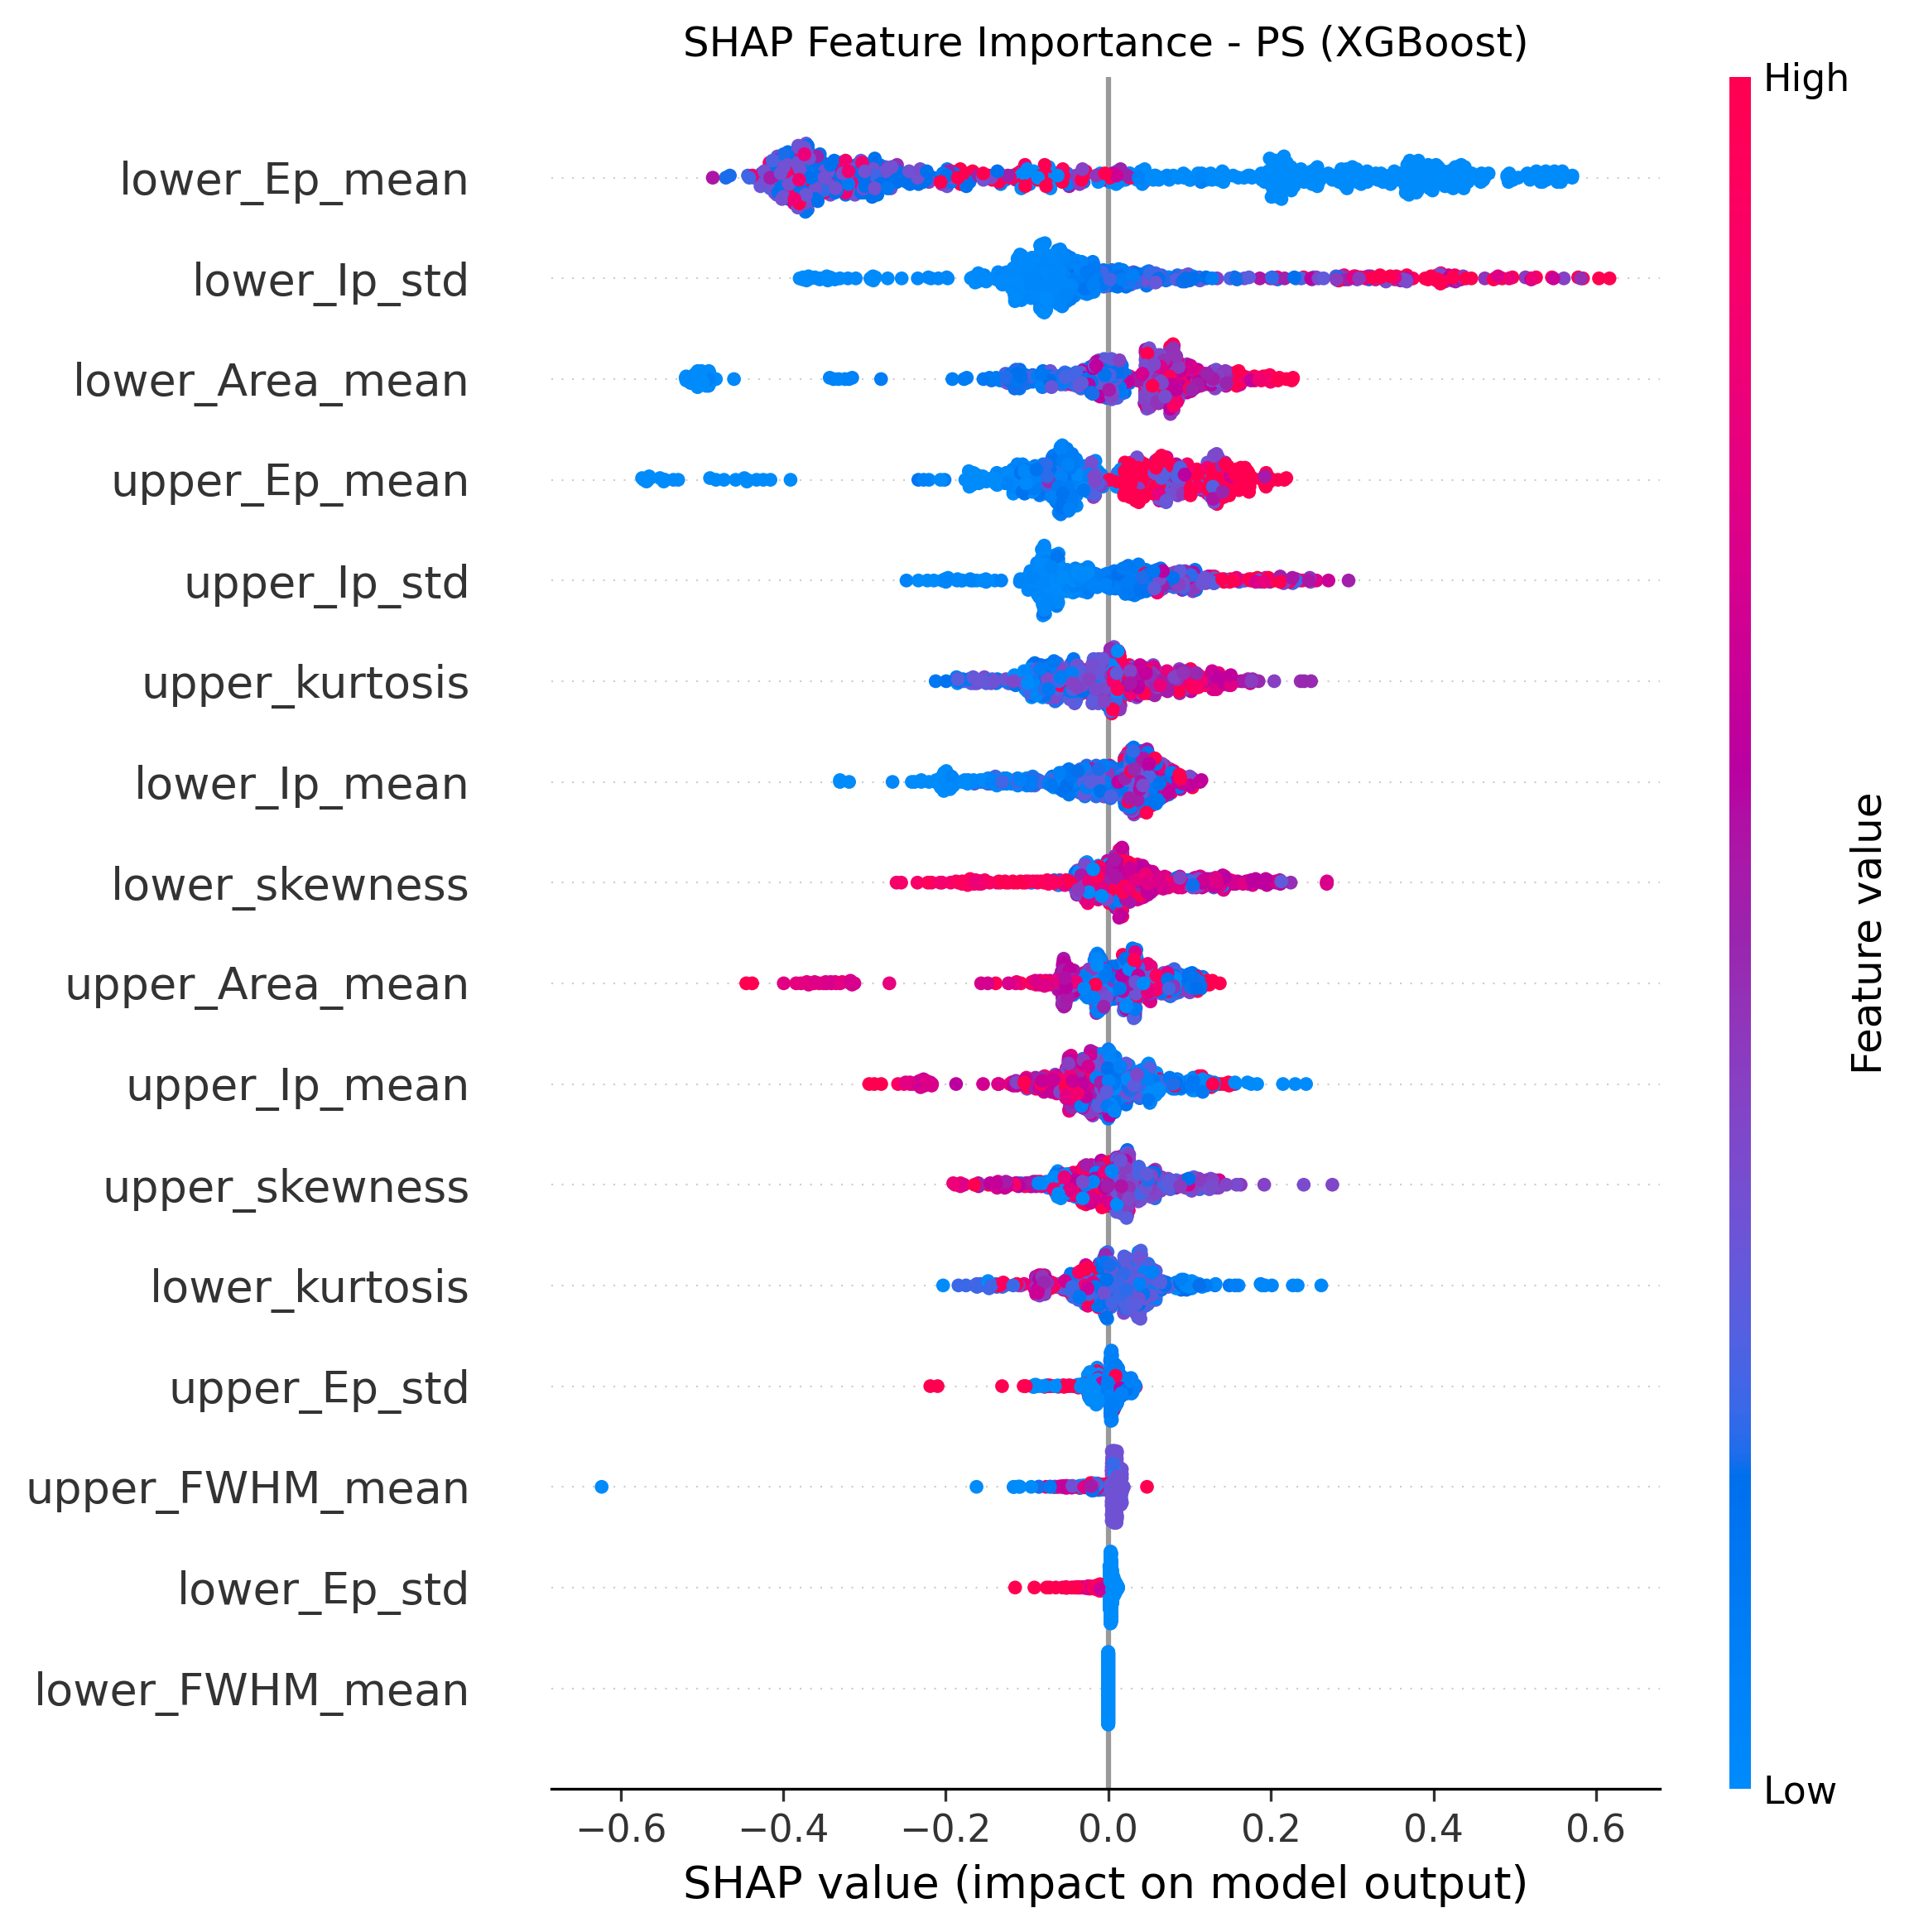
\includegraphics[width=\textwidth]{output/phase6_shap_ps.png}
        \caption{SHAP Summary Plot (PS)}
    \end{minipage}
\end{figure}

Interpretasi SHAP selaras dengan hukum fisikokimia dasar. Atribut \texttt{upper\_Ip\_mean} dan \texttt{upper\_Area\_mean} mendominasi keputusan model secara signifikan. Hal ini tervalidasi secara teoritis oleh Persamaan Randles-Sevcik, di mana *peak current* ($I_p$) dan luasan area di bawah kurva selalu berkorelasi linier dengan massa logam (molar) yang ter-oksidasi selama siklus voltammetri.

\section{KESIMPULAN}
Penelitian ini berhasil menyimpulkan keunggulan 	extbf{sensor rakitan LC (LecSens)} dibandingkan instrumen komersial EmStat4 (PS). Tiga temuan krusial yang dicatat:
\begin{enumerate}
    \item \textbf{Performa Regresi Superior:} Dengan memanfaatkan *Foundation Model* TabICLv2 dan metode ensemble XGBoost, instrumen LC mampu menembus skor determinasi $R^2$ hingga di atas 0.94, jauh meninggalkan skor puncak sensor PS.
    \item \textbf{Stabilitas Signal:} Penilaian stabilitas (*boxplot* antar *fold*) memperlihatkan bahwa rasio S/N (*Signal to Noise*) dari LC memfasilitasi algoritma *decision trees* untuk belajar secara optimal tanpa jatuh pada jeratan *overfitting* yang drastis.
    \item \textbf{Akurasi Rentang Rendah:} Kemampuan sensor LC dalam mendeteksi konsentrasi renik (0-10 ppm) terlihat secara jelas pada inspeksi plot residual, yang menjadikannya *cost-effective solution* untuk industri pemantauan kualitas perairan.
\end{enumerate}

\begin{thebibliography}{99}
\bibitem{dosen} Materi Perkuliahan Artificial Intelligence dan Data Science, Departemen Teknologi Informasi, Institut Teknologi Sepuluh Nopember, 2026.
\bibitem{sklearn} Pedregosa, F., et al. (2011). Scikit-learn: Machine Learning in Python. \textit{Journal of Machine Learning Research}, 12, 2825-2830.
\bibitem{xgboost} Chen, T., \& Guestrin, C. (2016). XGBoost: A Scalable Tree Boosting System. In \textit{Proceedings of the 22nd ACM SIGKDD}.
\bibitem{optuna} Akiba, T., Sano, S., Yanase, T., Ohta, T., \& Koyama, M. (2019). Optuna: A Next-generation Hyperparameter Optimization Framework. In \textit{KDD}.
\bibitem{pytorch} Paszke, A., et al. (2019). PyTorch: An Imperative Style, High-Performance Deep Learning Library. In \textit{NeurIPS}.
\bibitem{tabicl} TabICLv2: Zero-shot In-Context Learning for Tabular Data, Dokumentasi Teknis Model HuggingFace.
\bibitem{shap} Lundberg, S. M., \& Lee, S.-I. (2017). A Unified Approach to Interpreting Model Predictions. In \textit{Advances in Neural Information Processing Systems}.
\end{thebibliography}

\end{document}
